\documentclass[12pt]{article}
\usepackage{sbc-template}
\usepackage{graphicx,url}
\usepackage[brazil]{babel}   
\usepackage[utf8]{inputenc}
\usepackage{graphicx}
\usepackage{subfigure}
\usepackage{amsmath}
\usepackage{bbm}
\usepackage{cite}
\usepackage{listings}
\usepackage{color}
\usepackage{indentfirst}
\usepackage{float}

\lstset{language=Python,
                basicstyle=\ttfamily,
                keywordstyle=\color{blue}\ttfamily,
                stringstyle=\color{red}\ttfamily,
                commentstyle=\color{green}\ttfamily,
                morecomment=[l][\color{magenta}]{\#}
}


\title{Visualização da Dados de Informações Extraídas da Web - Um estudo sobre Conteúdo Popular Japonês}
\author{Gabriel Fontenelle\inst{1}}
\address 
{Centro Universitário Senac - Campus Santo Amaro
  (SENAC-SP)\\
  Av. Engenheiro Eusébio Stevaux, 823 -- São Paulo -- CEP 04696-000 -- SP -- Brasil
%\nextinstitute
%  Departamento de Tecnologia da Informação\\
%  Bacharelado em Ciência da Computação
  \email{{colecionador.gabriel@gmail.com}}
}

\begin{document} 
\maketitle

\begin{abstract}

This work 
\end{abstract}
     
\begin{resumo} 


Este trabalho apresenta um estudo sobre coleções de itens da cultura popular japonesa na forma de visualização de dados obtidos por meio de crawleamento de diversos websites.

\end{resumo}


\section{Introdução}

O foco deste trabalho é a criação de Visualização de dados a partir de informações extraídas de websites que disponibilizam quantidade de dados maciça.

Para a criação da Visualização de Dados foi escolhido o tema: Cultura Popular Japonesa. O tema é abrangente e poderíamos obter e utilizar informações sobre os seus diversos produtos comercializados: mangás, animes, Light Novels, Visual Novels e outros bens de consumo derivados como braceletes e "Figuras de Ação" que são colecionados por colecionadores em grande parte do mundo ocidental.

A Cultura Popular Japonesa é conhecida pelo desenvolvimento de animações, revistas em quadrinhos e gêneros literários influenciados por um estilo de desenho único focado nas expressões de suas personagens. Nos países ocidentais as animações, histórias em quadrinhos originadas no Japão são nomeadas respectivamente como anime e manga.
Com a popularização de jogos eletrônicos surgiram dois gêneros literários no Japão: Light Novel e Visual Novel. Light Novel é um gênero literário caracterizado pelo menor número de páginas e escrita mais clara utilizando-se em maior parte de Furiganas, possui histórias fluídas com desenvolvimento rápido muitas vezes utilizando-se de efeitos sonoros para ilustrar situações em vez de uma descrição completa da situação, como exemplo a saída de uma personagem de um quarto com uma batida grosseira da porta pode demonstrada apenas mencionando que a personagem saiu o efeito sonoro realizado na porta. Light Novel também é caracterizado pelas ilustrações de algumas cenas e por isso pode ser comparado a Graphic Novels (Histórias em inglês que possuem algumas páginas ilustradas). Visual Novel também é formado por ilustrações e textos mais claros de serem entendidos que livros tradicionais, mas diferente de Light Novel se assemelham mais a um jogo de computador em que decisões dos jogadores podem alterar o rumo da história.

Neste trabalho as informações foram extraídas de diversos websites com o uso de biblioteca de Crawler e salvas em um banco de dados previamente modelado para geração posterior de diversas visualizações de dados. 

Visualização de dados é uma forma de comunicar visualmente informações que de outro modo não seriam facilmente identificáveis.


\section{Desenvolvimento}

\subsection{Websites para extração de dados}

O tema escolhido é abrangente assim como possui diversos websites que poderíamos utilizar para a extração de informações. Focamo-nos na visualização de dados ilustrando informações sobre Coleções e seus produtos derivados como artigos decorativos e "Figuras de Ação" baseados em personagens presentes nas Coleções. 

Os websites escolhidos se encontram abaixo, a escolha de websites com informações reduntantes é proposital uma vez que não poderíamos garantir a conectividade com os sites durante o desenvolvimento deste trabalho. 

\begin{itemize}
\item http://mangaupdates.com/ (Para extração de informação de Mangás e Light Novels)
\item http://myfigurecollection.net/ (Para extração de informações de Mangás, "Figuras de Ação" e Outros Produtos)
\item http://www.animecharactersdatabase.com/ (Para extração de informações de Jogos para computador, animes e personagens)
\end{itemize}

Os sites escolhidos possuem informações principalmente no idioma inglês mas também fornecem algumas informações em outros idiomas, como os títulos de mangás e animes em Japonês ou até mesmo Português. Para aproveitarmos essas informações o Banco de Dados foi modelado a permitir múltiplos idiomas. 

\subsection{Modelagem do Banco de Dados}

Antes sequer de prosseguirmos com o desenvolvimento do sistema de extração de informações dos websites optamos por criar um Banco de Dados normalizado para quando fossemos extrair e salvar as informações desses websites, os dados já seriam salvos em uma estrutura relacionado e normalizado.

Foi portanto desenvolvido o Modelo Conceitual, Modelo Relacional e Modelo Lógico do Banco de Dados.

Para o Sistema de Banco de Dados foi escolhido o PostgreSQL, sob licença BSD, disponível para diversos sistemas operacionais, possuindo Transações que seguem o modelo ACID com recursos como Commit e Rollback e opção para criação de atributos com tipos de dados personalizados. 

Este trabalho faz uso extenso de Commit e Rollback no tratamento de erros, assim transações com falhas parciais são descartadas evitando o salvamento de conteúdo incompleto.

%Como para extração dos dados dos websites escolhidos é necessário 
%Com a mentalidade que é melhor pegar todas as informações disponibilizadas pois é melhor ter que precisar e não ter, foi modelado um Banco de Dados que expandiu o conceito original e possibilita a inserção de dados relacionais para armazenamento de músicas, vídeos, livros e diversas informações associadas. 

\subsubsection{Modelo Conceitual}

O conceito inicial de armazenar informações relacionais sobre itens da Cultura Popular Japonesa resultou em um Modelo Conceitual em que se poderia armazenar informações de mangás, animes e "Figuras de Ação". Esse conceito original foi expandido para possibilitar a inserção de dados relacionais sobre músicas, jogos de computador, vídeos, livros e diversas informações associadas a Coleções. 

Com a expansão do tipo de informação a ser salva no Banco de Dados a criação do Modelo Conceitual se tornou complexa, além do tradicional uso de atributos e relacionamentos foram utilizados conceito de especialização/generalização e associação. 

Como a estrutura do Modelo Conceitual é complexa e grande dividimos sua ilustração em partes e para melhor compreensão antes de apresentarmos cada parte mostraremos um diagrama mais simples abrangendo as principais entidades do Modelo Conceitual:

\begin{figure}[H]
\centering
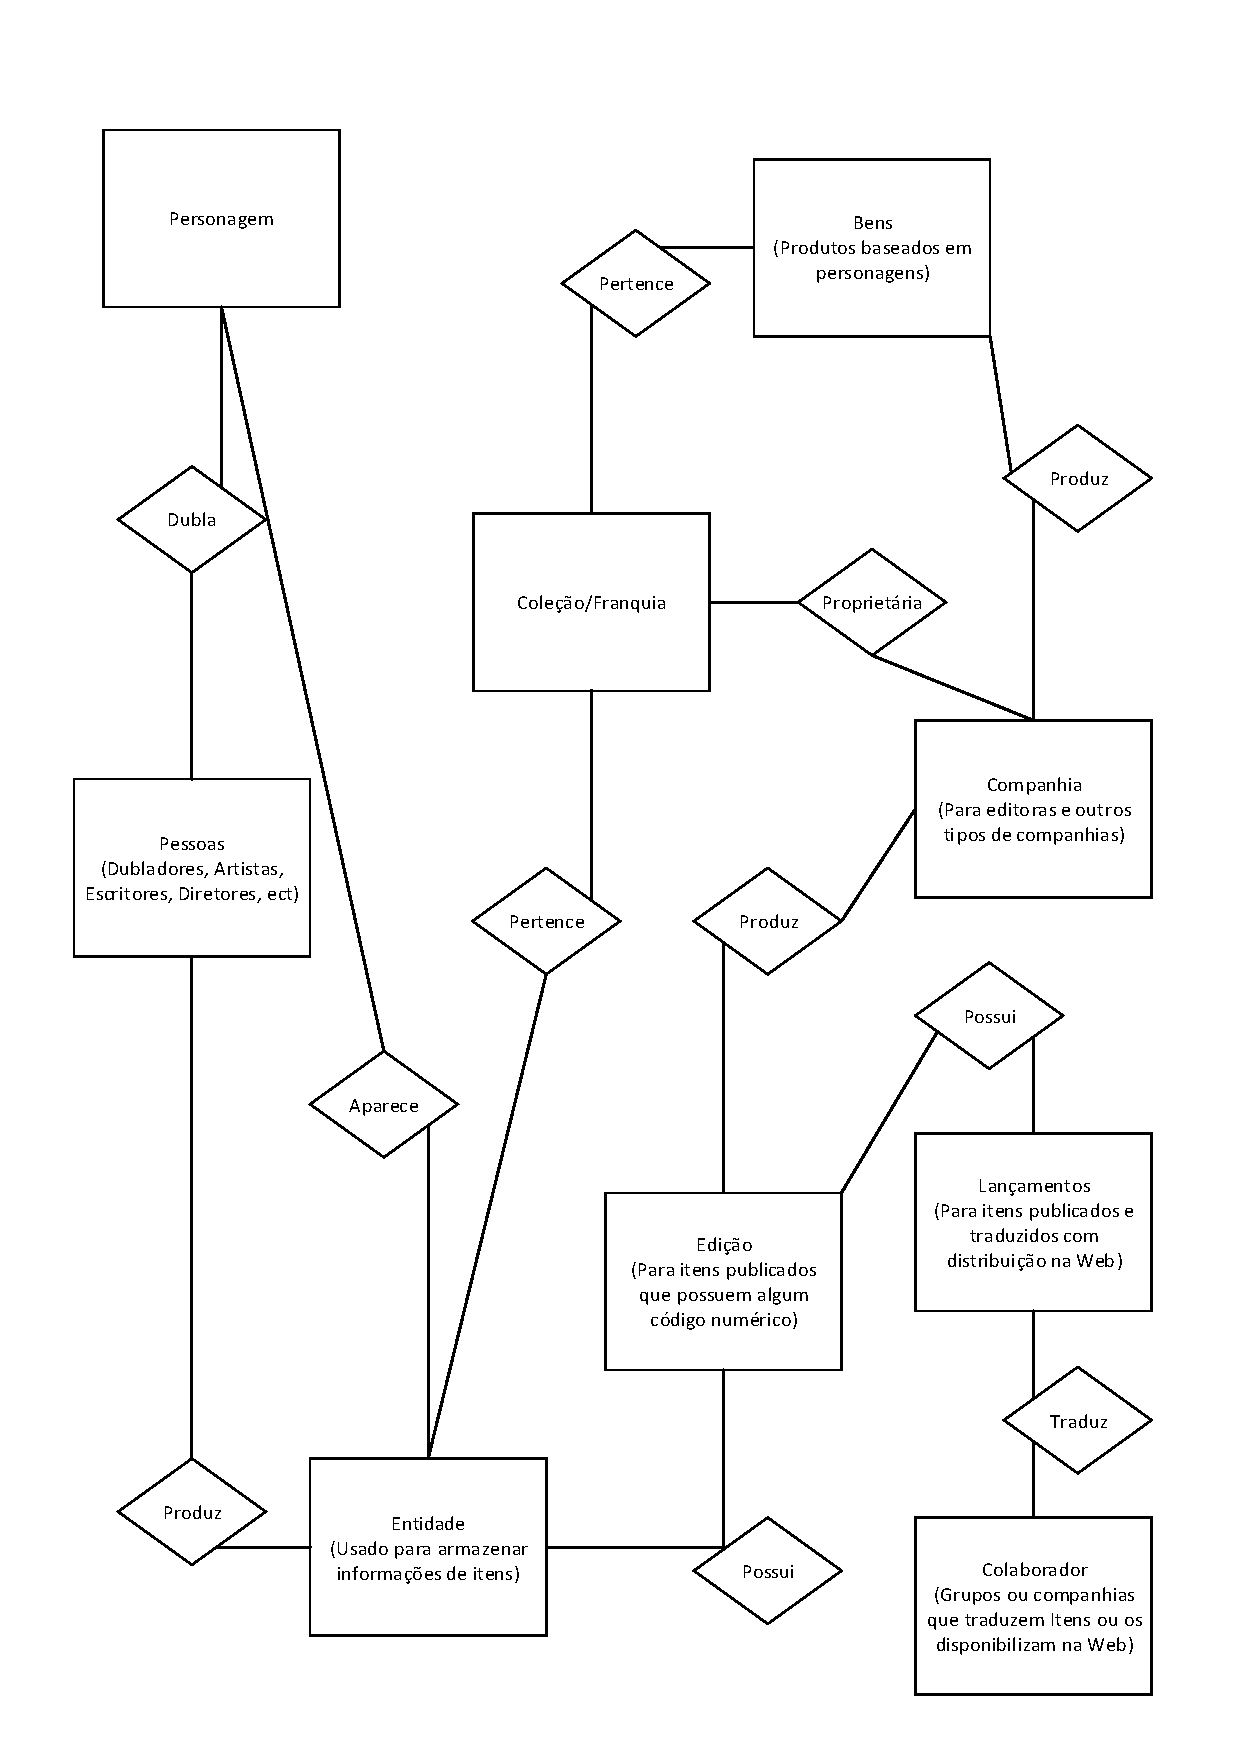
\includegraphics[width=.80\textwidth]{MER_-_General.pdf}
\caption{Modelo Conceitual resumido com os nomes das principais entidades em português. Na implementação do Modelo Lógico foram utilizados nomes em inglês.} \label{hash}
\end{figure}


A seguir pode ser observado as entidades e seus relacionamentos de forma mais detalhada. As entidades na cor laranja serão detalhadas mais a frente.

\begin{figure}[H]
\centering
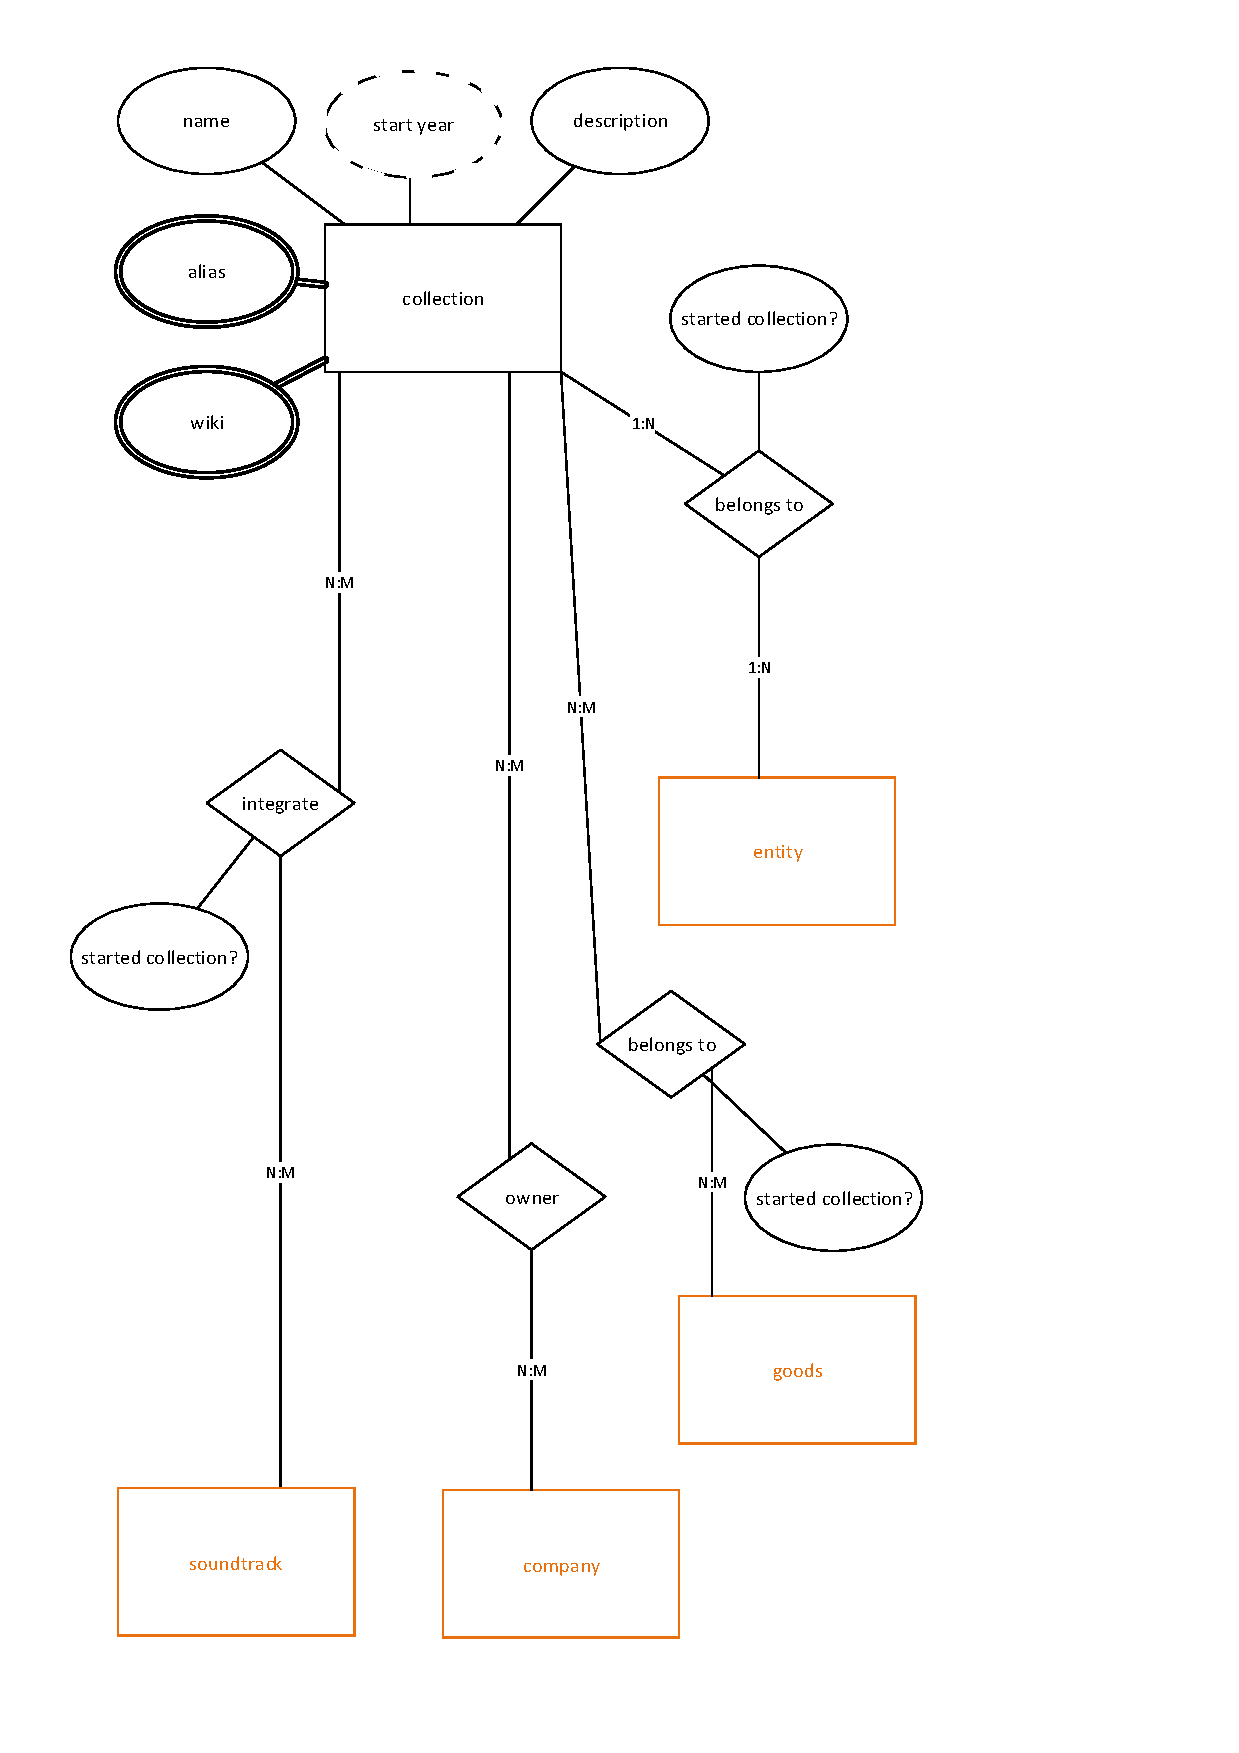
\includegraphics[width=.80\textwidth]{MER_-_Collection.pdf}
\caption{Entidade responsável por armazenar informações de coleções.} \label{collection}
\end{figure}


\begin{figure}[H]
\centering
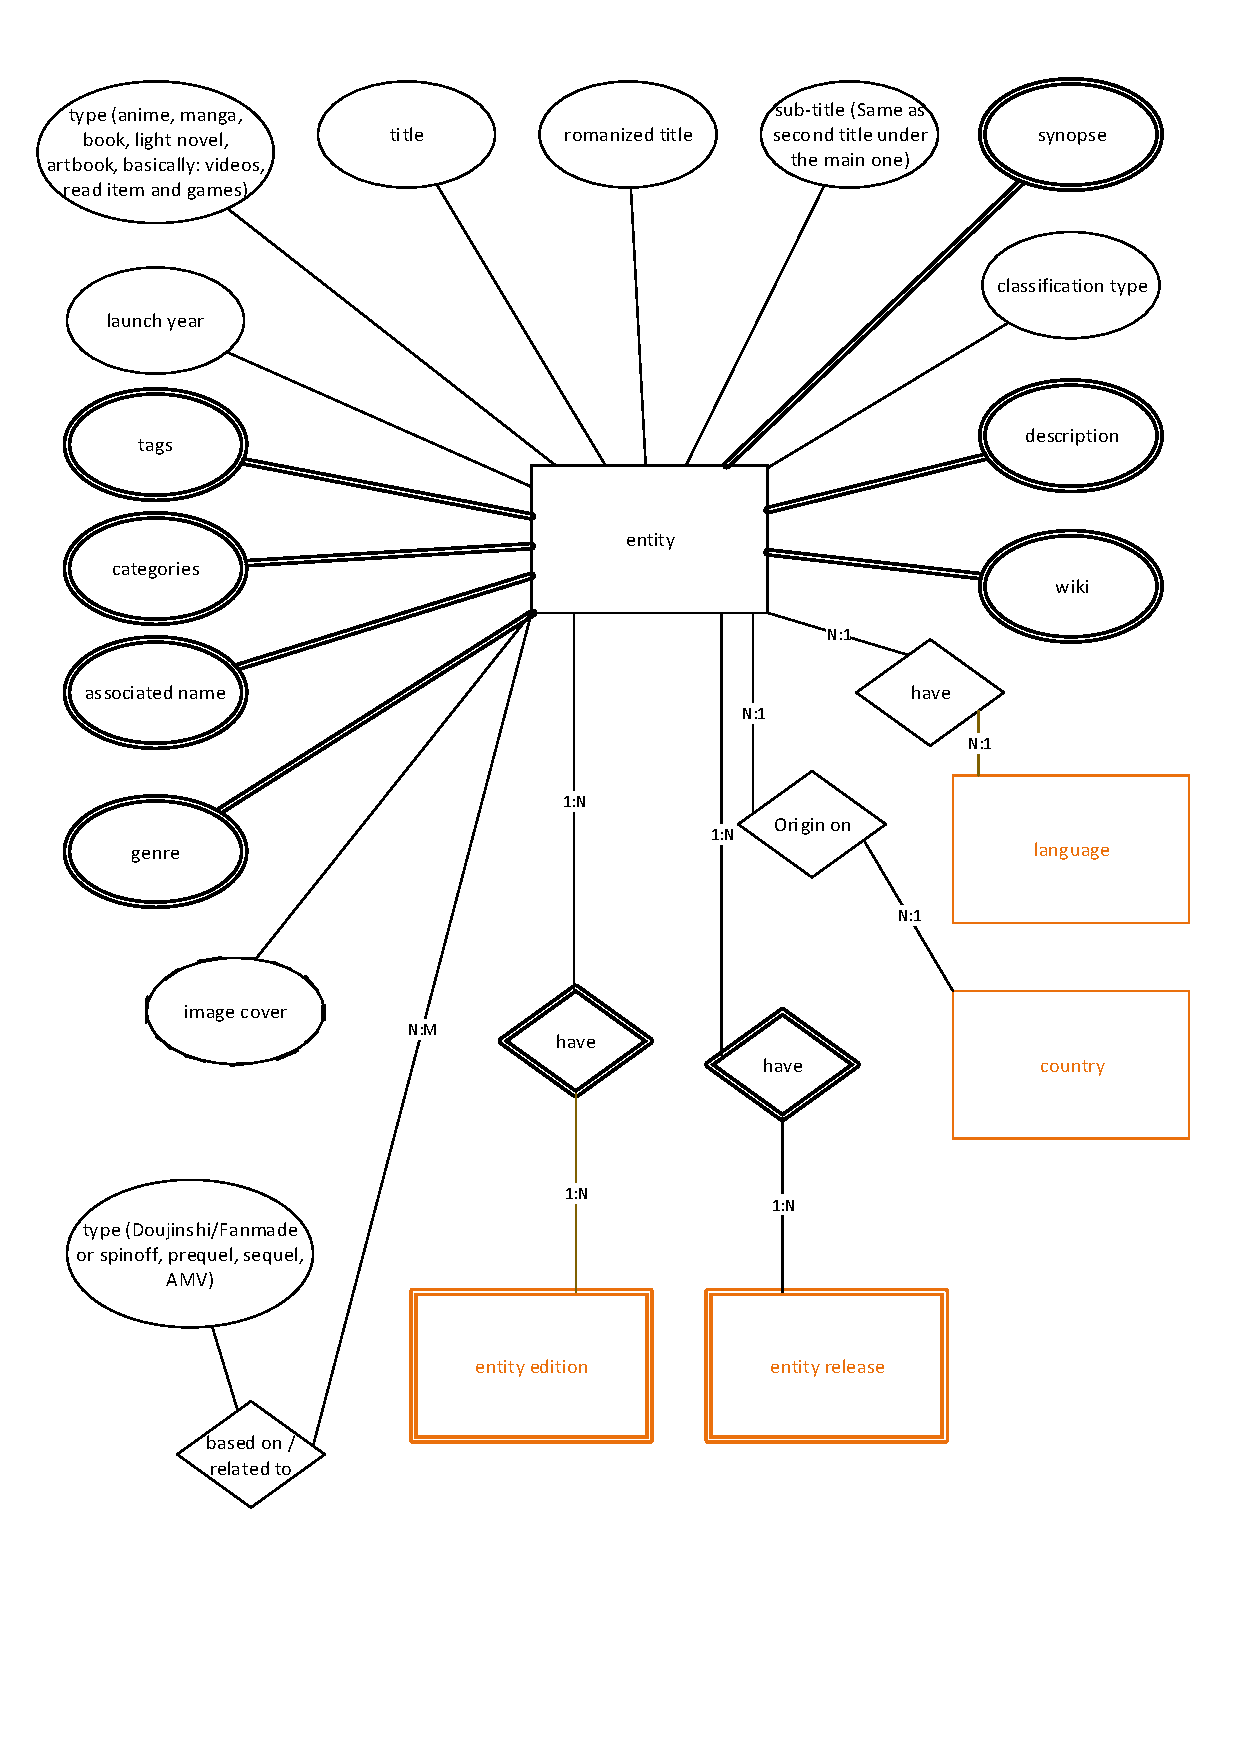
\includegraphics[width=.80\textwidth]{MER_-_Entity.pdf}
\caption{Entidade "Entity" é responsável por armazenar conteúdo como Vídeos, Livros e Jogos.} \label{entity}
\end{figure}

\begin{figure}[H]
\centering
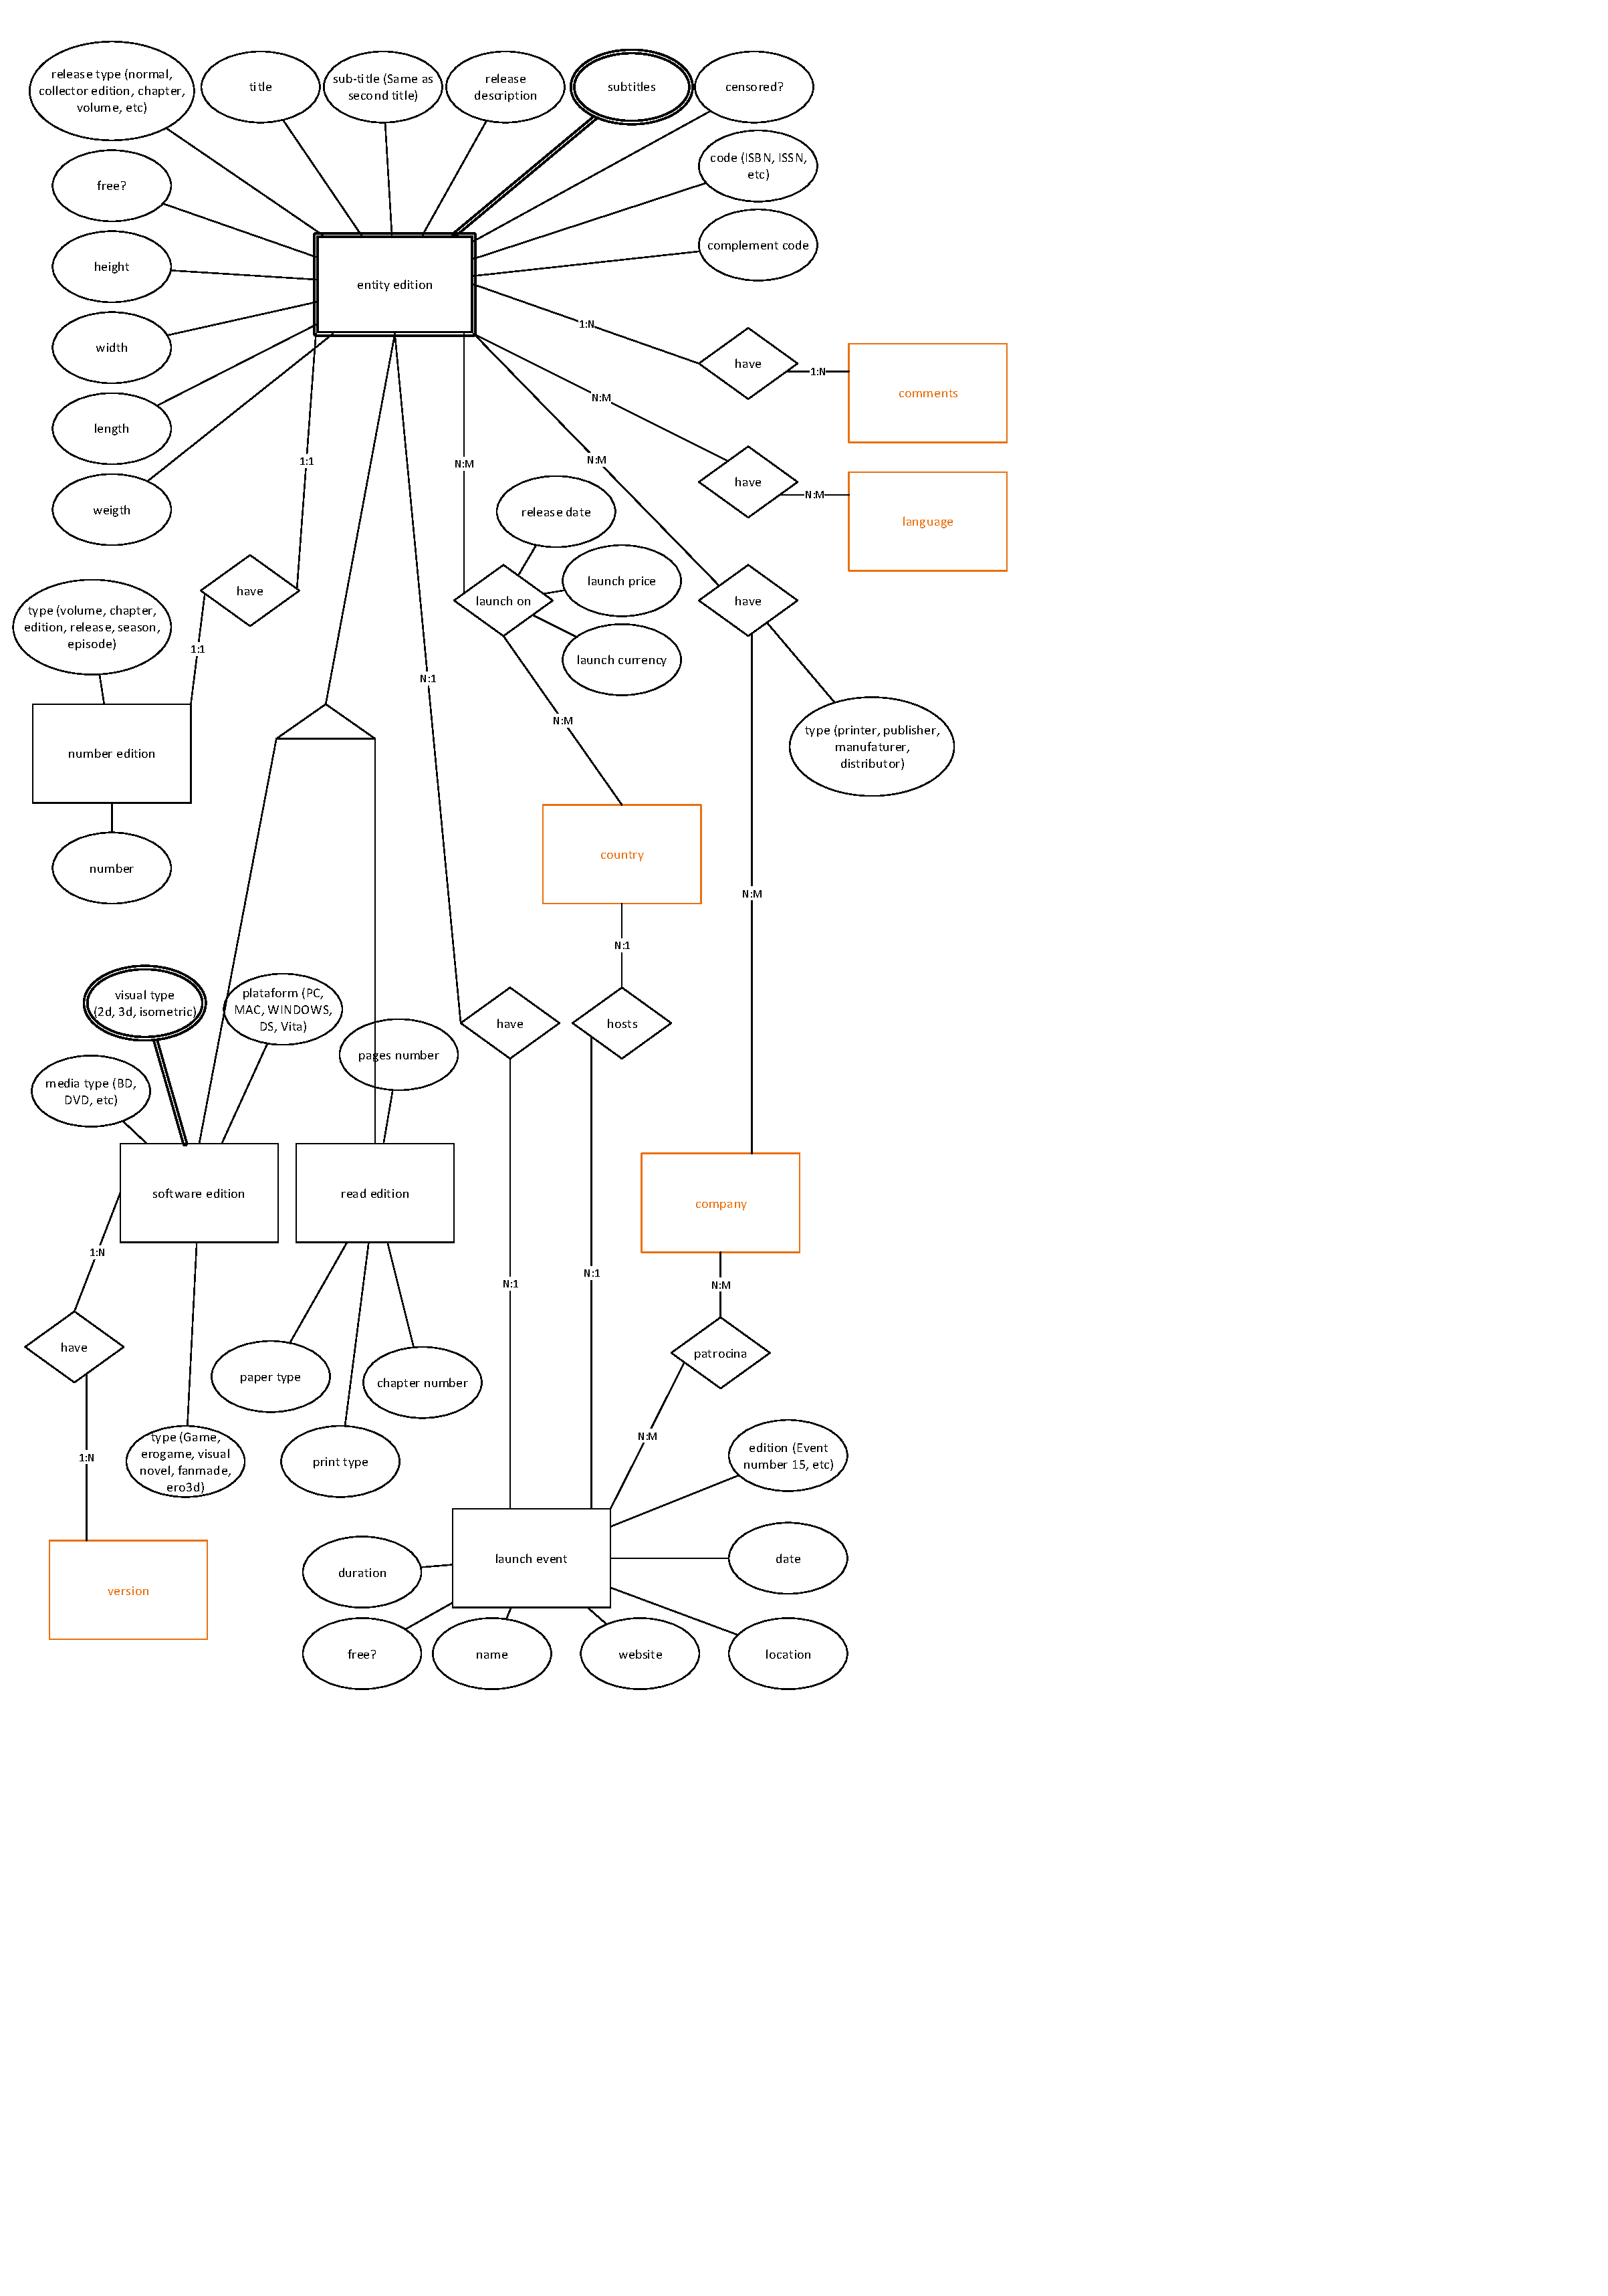
\includegraphics[width=.80\textwidth]{MER_-_Edition.pdf}
\caption{Entidade "Edition" é responsável por armazenar informações de itens de "Entity" que possuem publicação física. "Edition" se especializa em "Software Edition" para armazenamento de informações especificas a softwares e "Read Edition" para armazenamento de informações de livros e revistas} \label{edition}
\end{figure}

\begin{figure}[H]
\centering
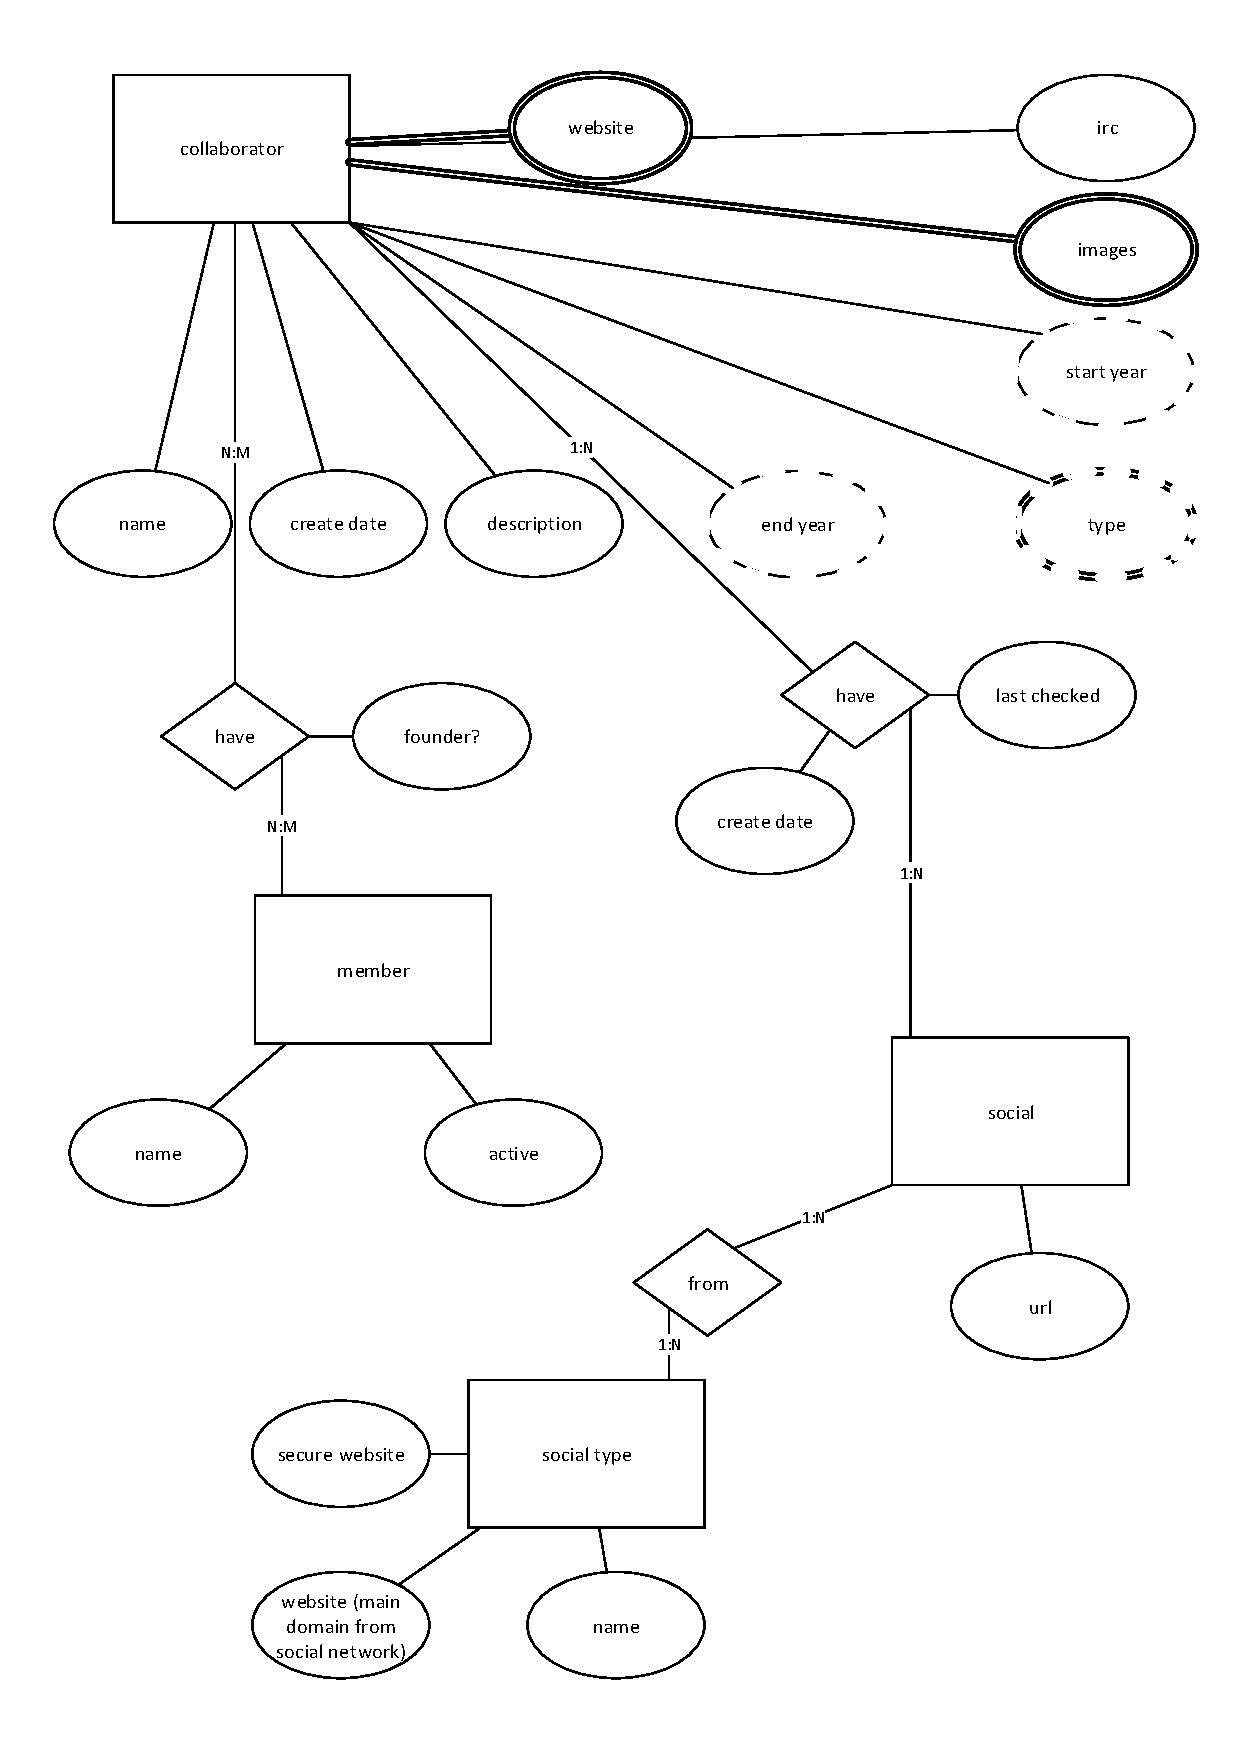
\includegraphics[width=.80\textwidth]{MER_-_Collaborator_Social.pdf}
\caption{Entidades com informações sobre Colaboradores que traduzem conteúdo Popular Japonês e suas redes sociais.} \label{collaborator}
\end{figure}

\begin{figure}[H]
\centering
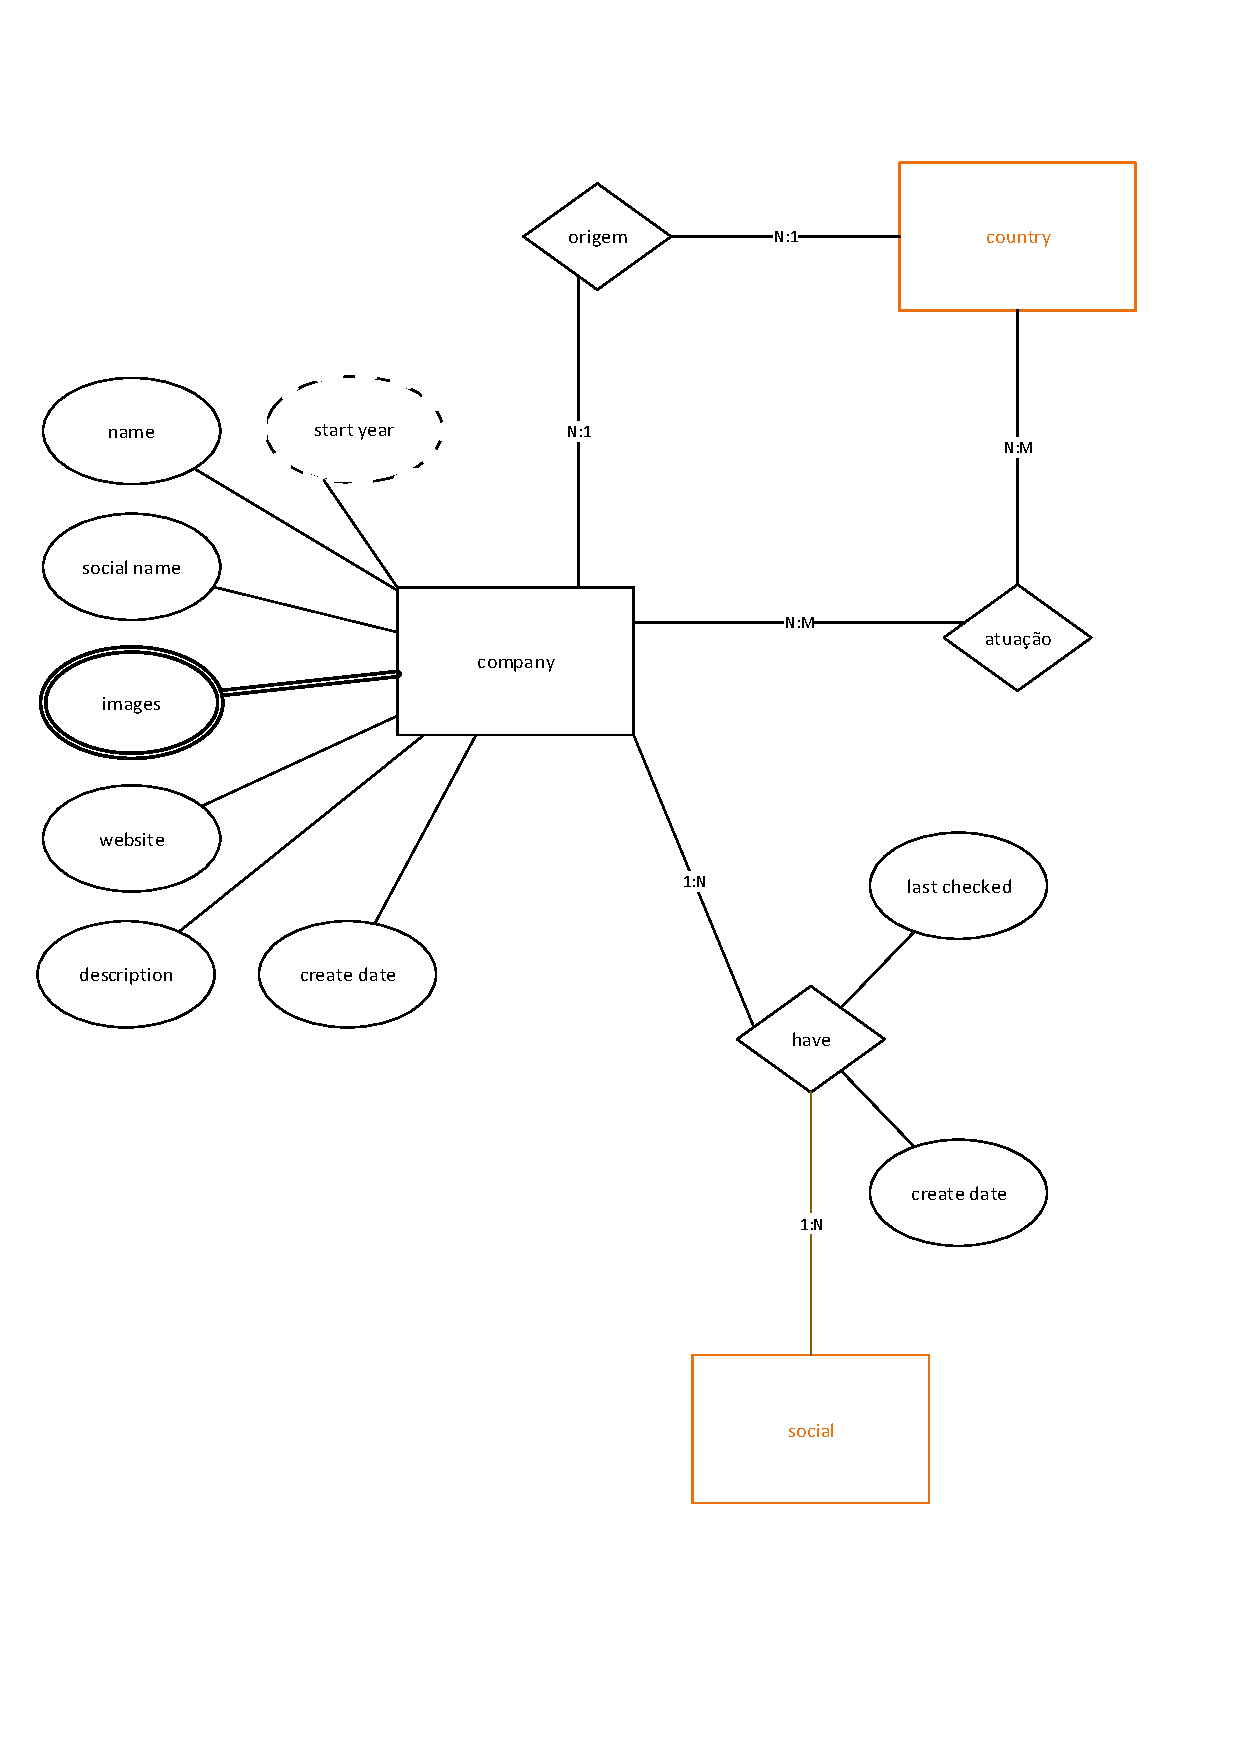
\includegraphics[width=.80\textwidth]{MER_-_Company.pdf}
\caption{Entitidade "Company" é responsável por arzenar informações de empresas. A atividade que a empresa exerce é definida no relacionamento.} \label{company}
\end{figure}

\begin{figure}[H]
\centering
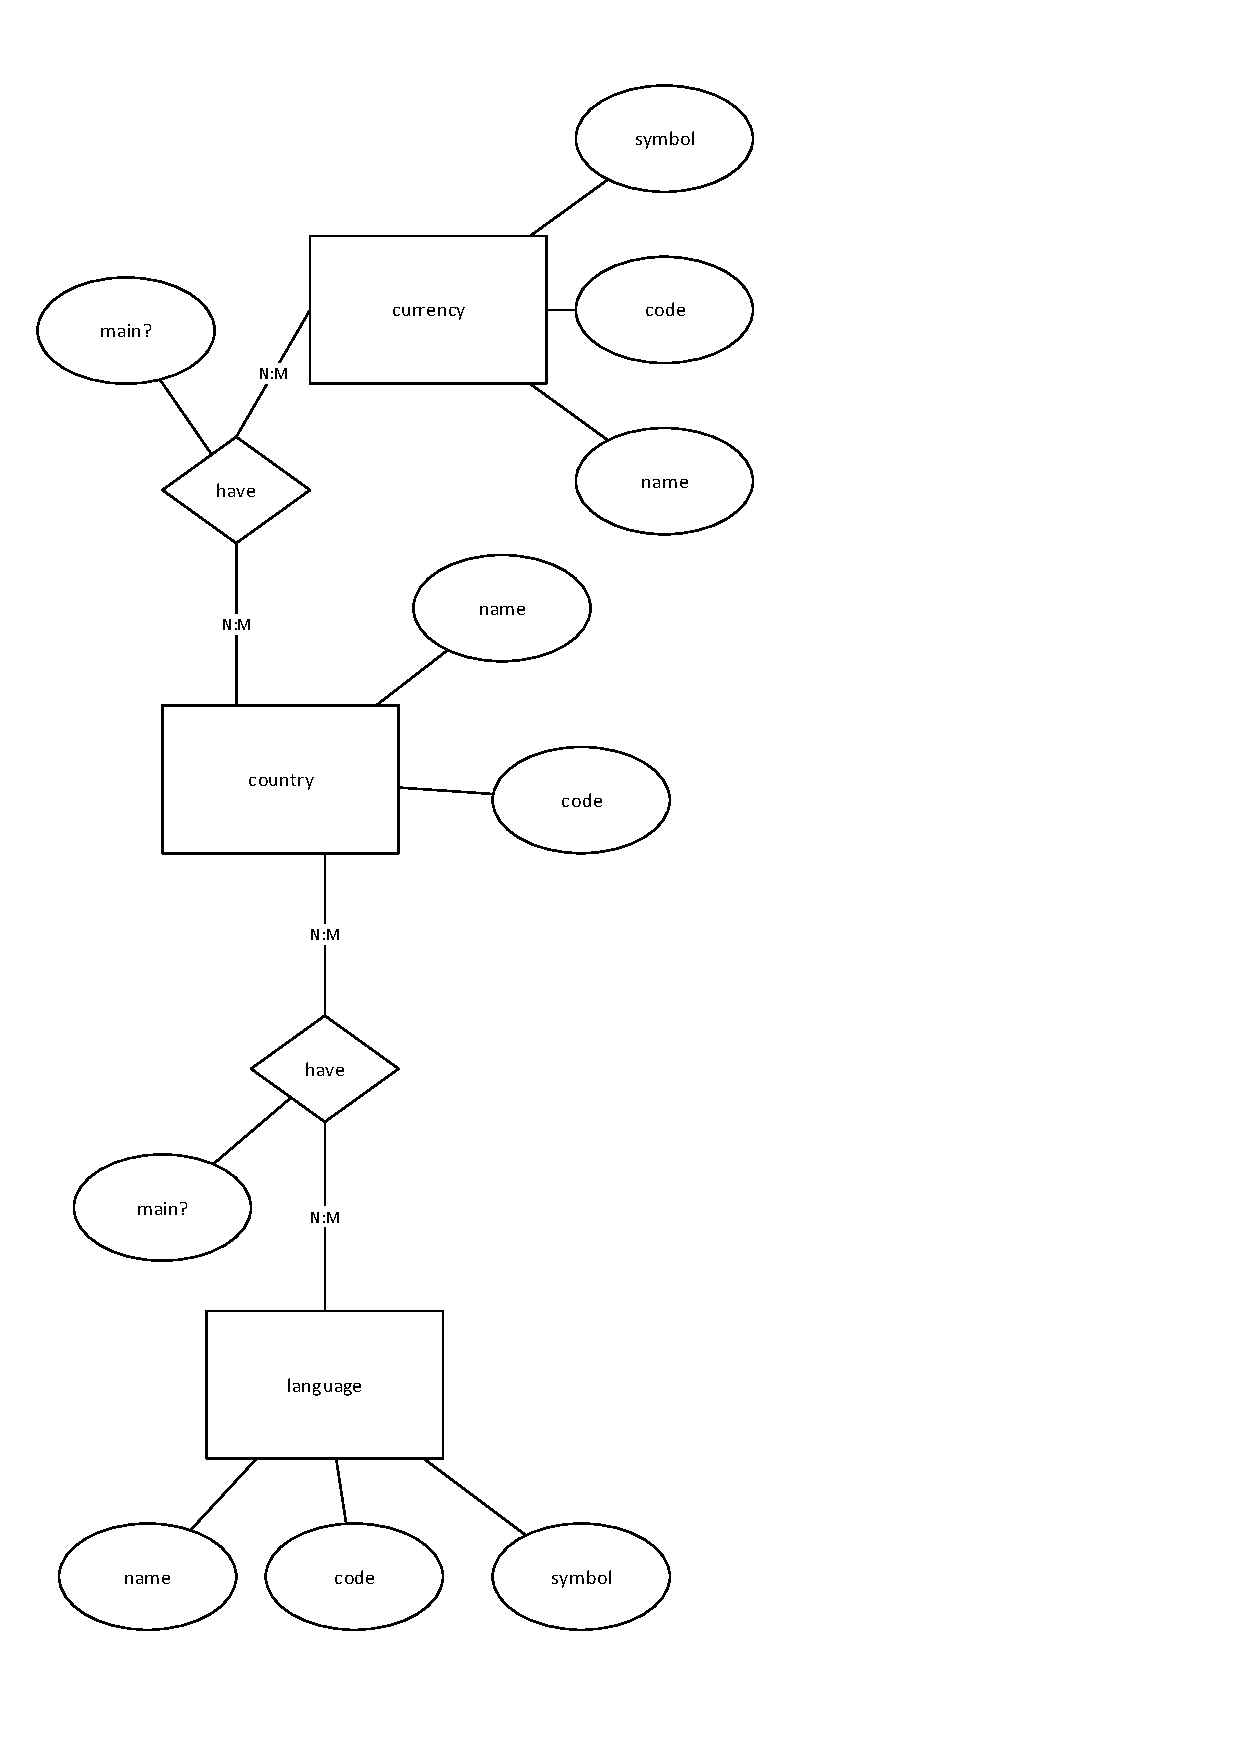
\includegraphics[width=.80\textwidth]{MER_-_Country-Language-Currency.pdf}
\caption{Entidades responsáveis pelo armazenamento de informações de Países, seus idiomas e suas moedas.} \label{hash}
\end{figure}

Como exemplo de especialização/generalização temos no Modelo Conceitual a entitidade Goods onde bens de consumo como braceletes, posters, chaveiros são armazenados. Essa entidade se especializa na entidade Figure que armazena informações de bens conhecidos como figures ou action figures, são artigos colecionáveis em Três Dimensões de Personagens de animes, mangás, video games e light novels,
 que possuem informações extras além das contidas em Goods como escala e versão de lançamento.

\begin{figure}[H]
\centering
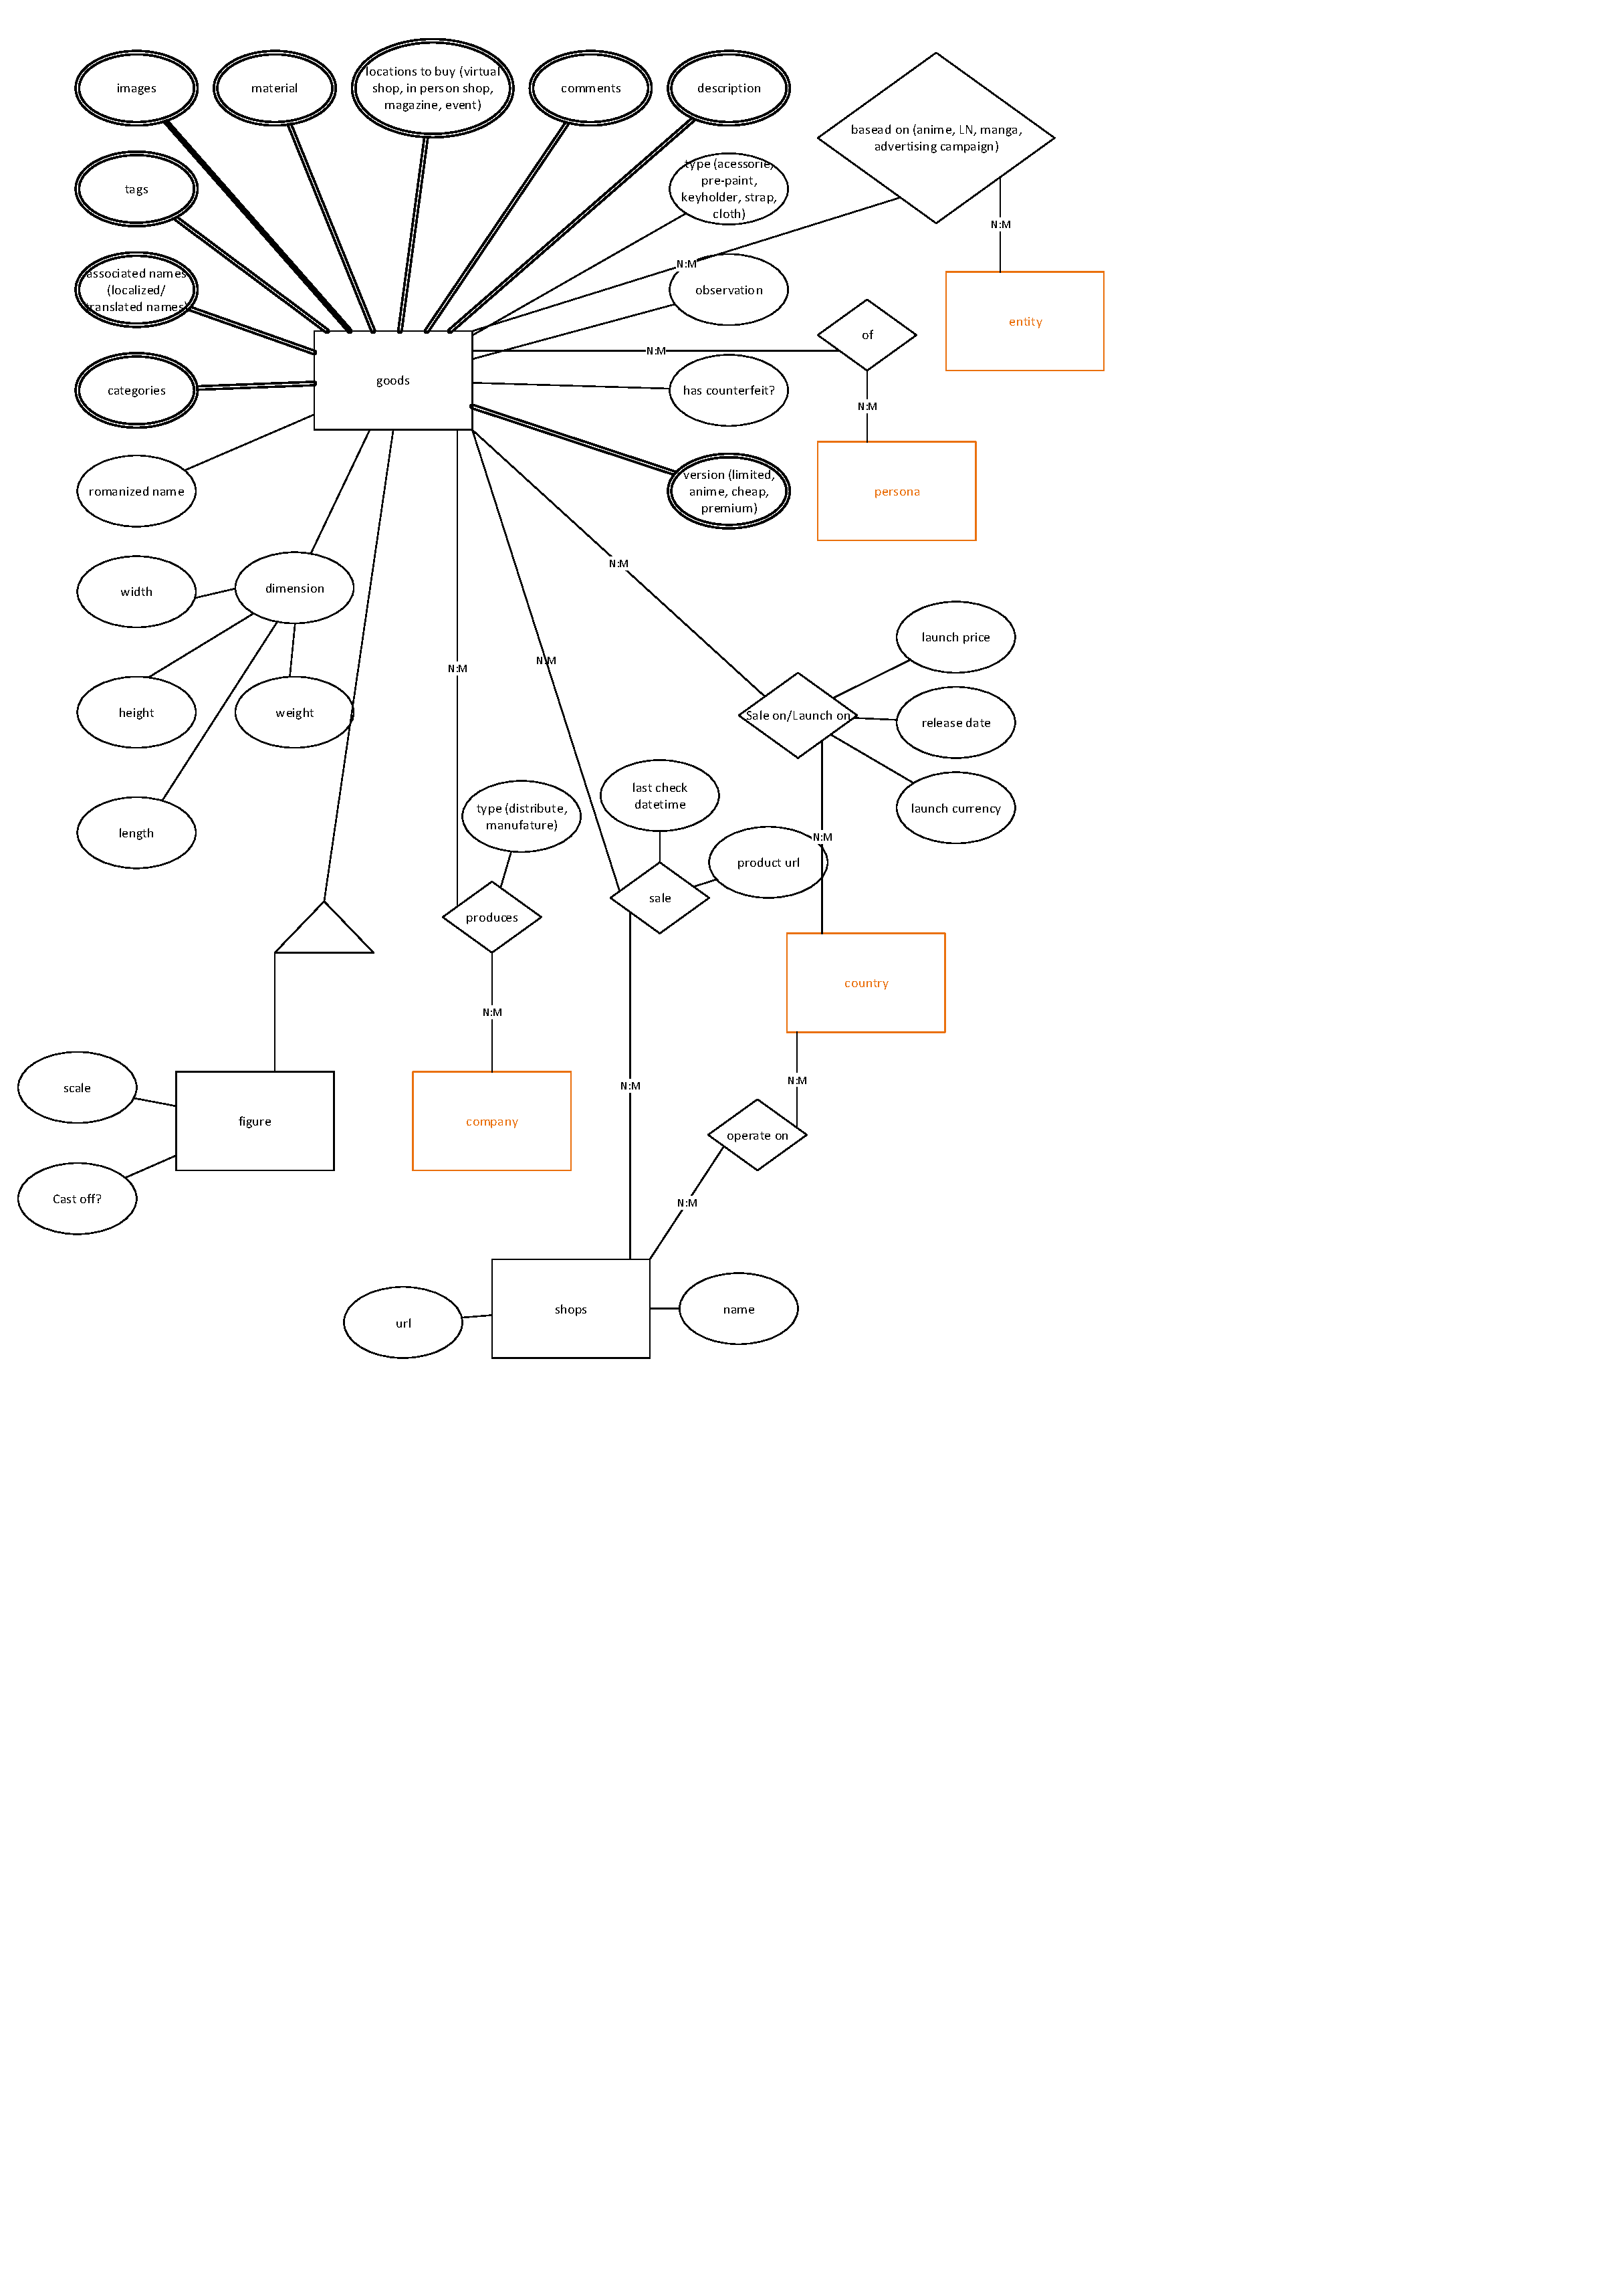
\includegraphics[width=.80\textwidth]{MER_-_Goods.pdf}
\caption{Entidade "Goods" se especializa em "Figure".} \label{hash}
\end{figure}

\begin{figure}[H]
\centering
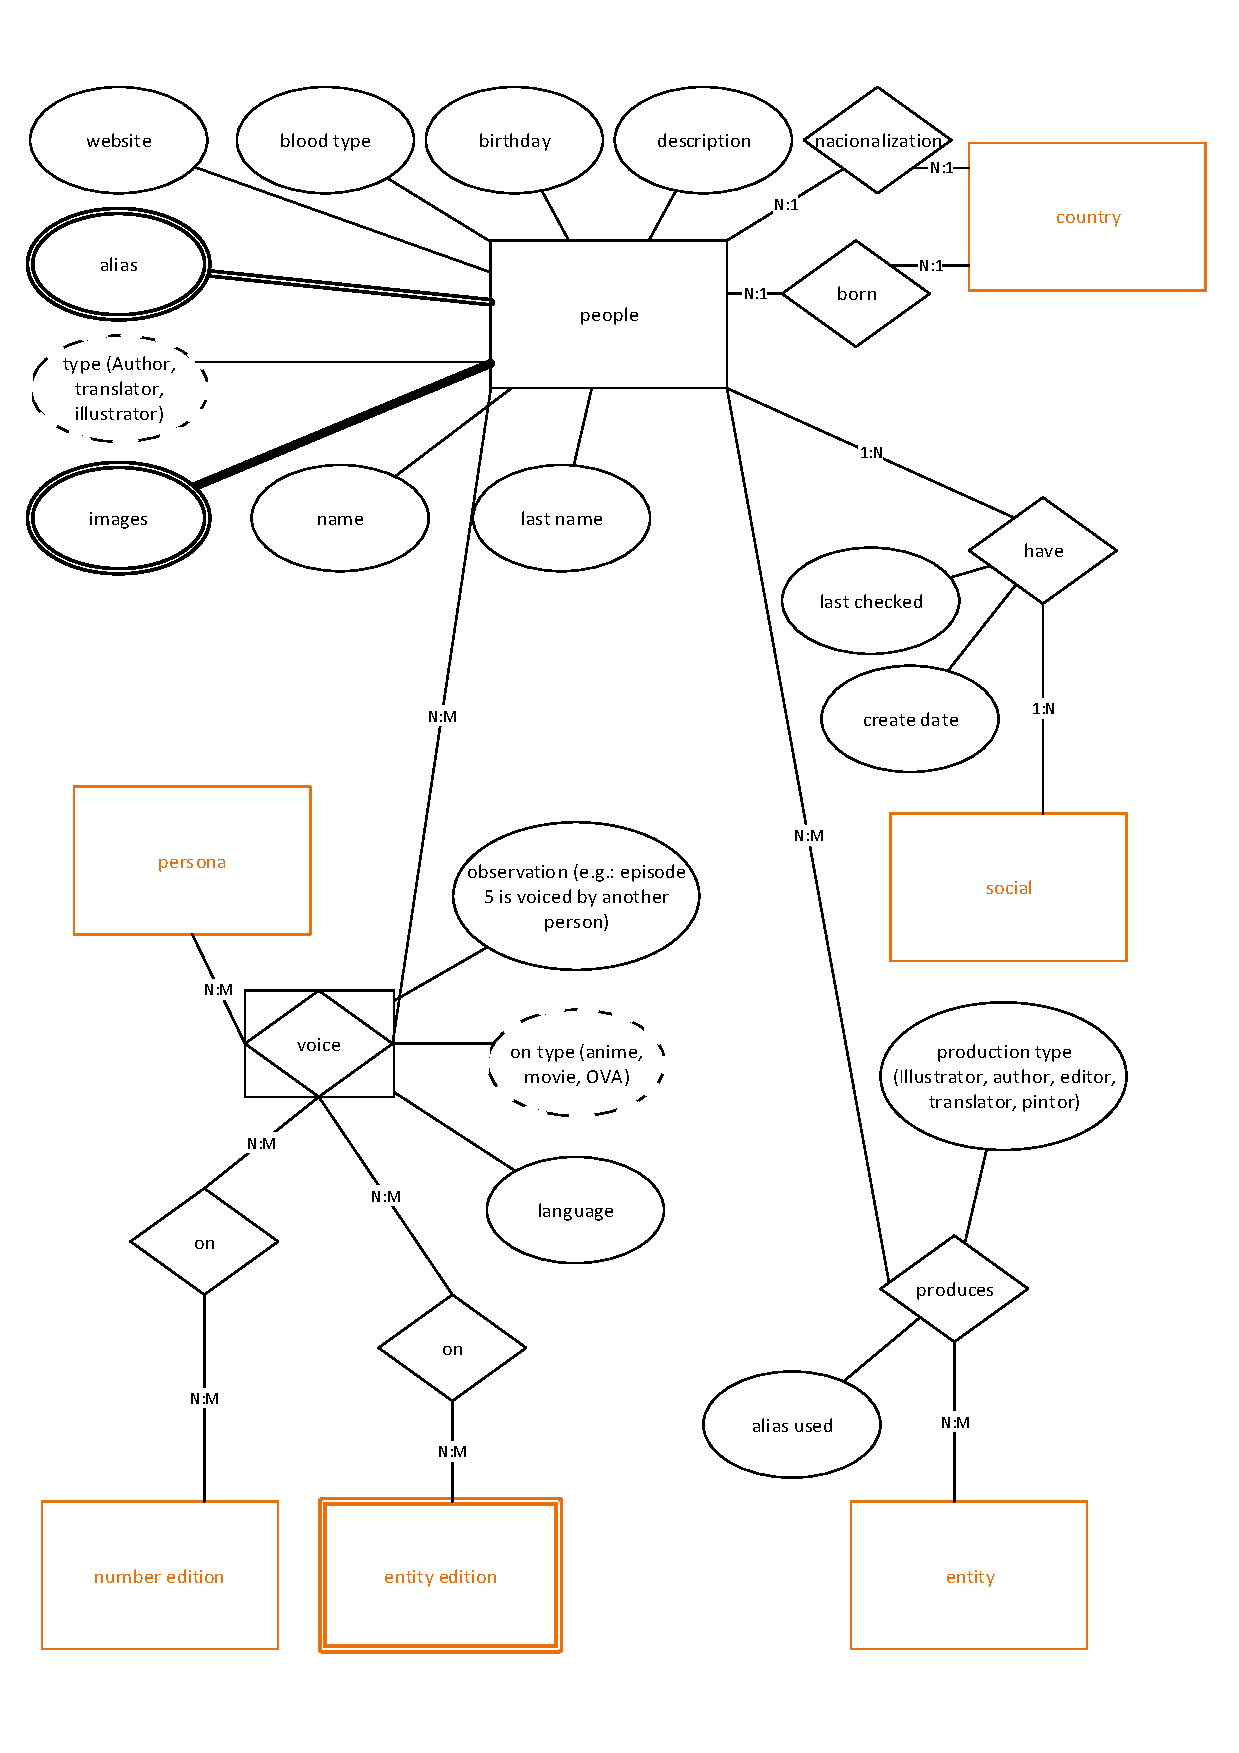
\includegraphics[width=.80\textwidth]{MER_-_People.pdf}
\caption{Entidades responsáveis pelo armazenamento de informações de pessoas. A atividade exercida por uma pessoa em um determinado trabalho é definida no relacionamento.} \label{hash}
\end{figure}

\begin{figure}[H]
\centering
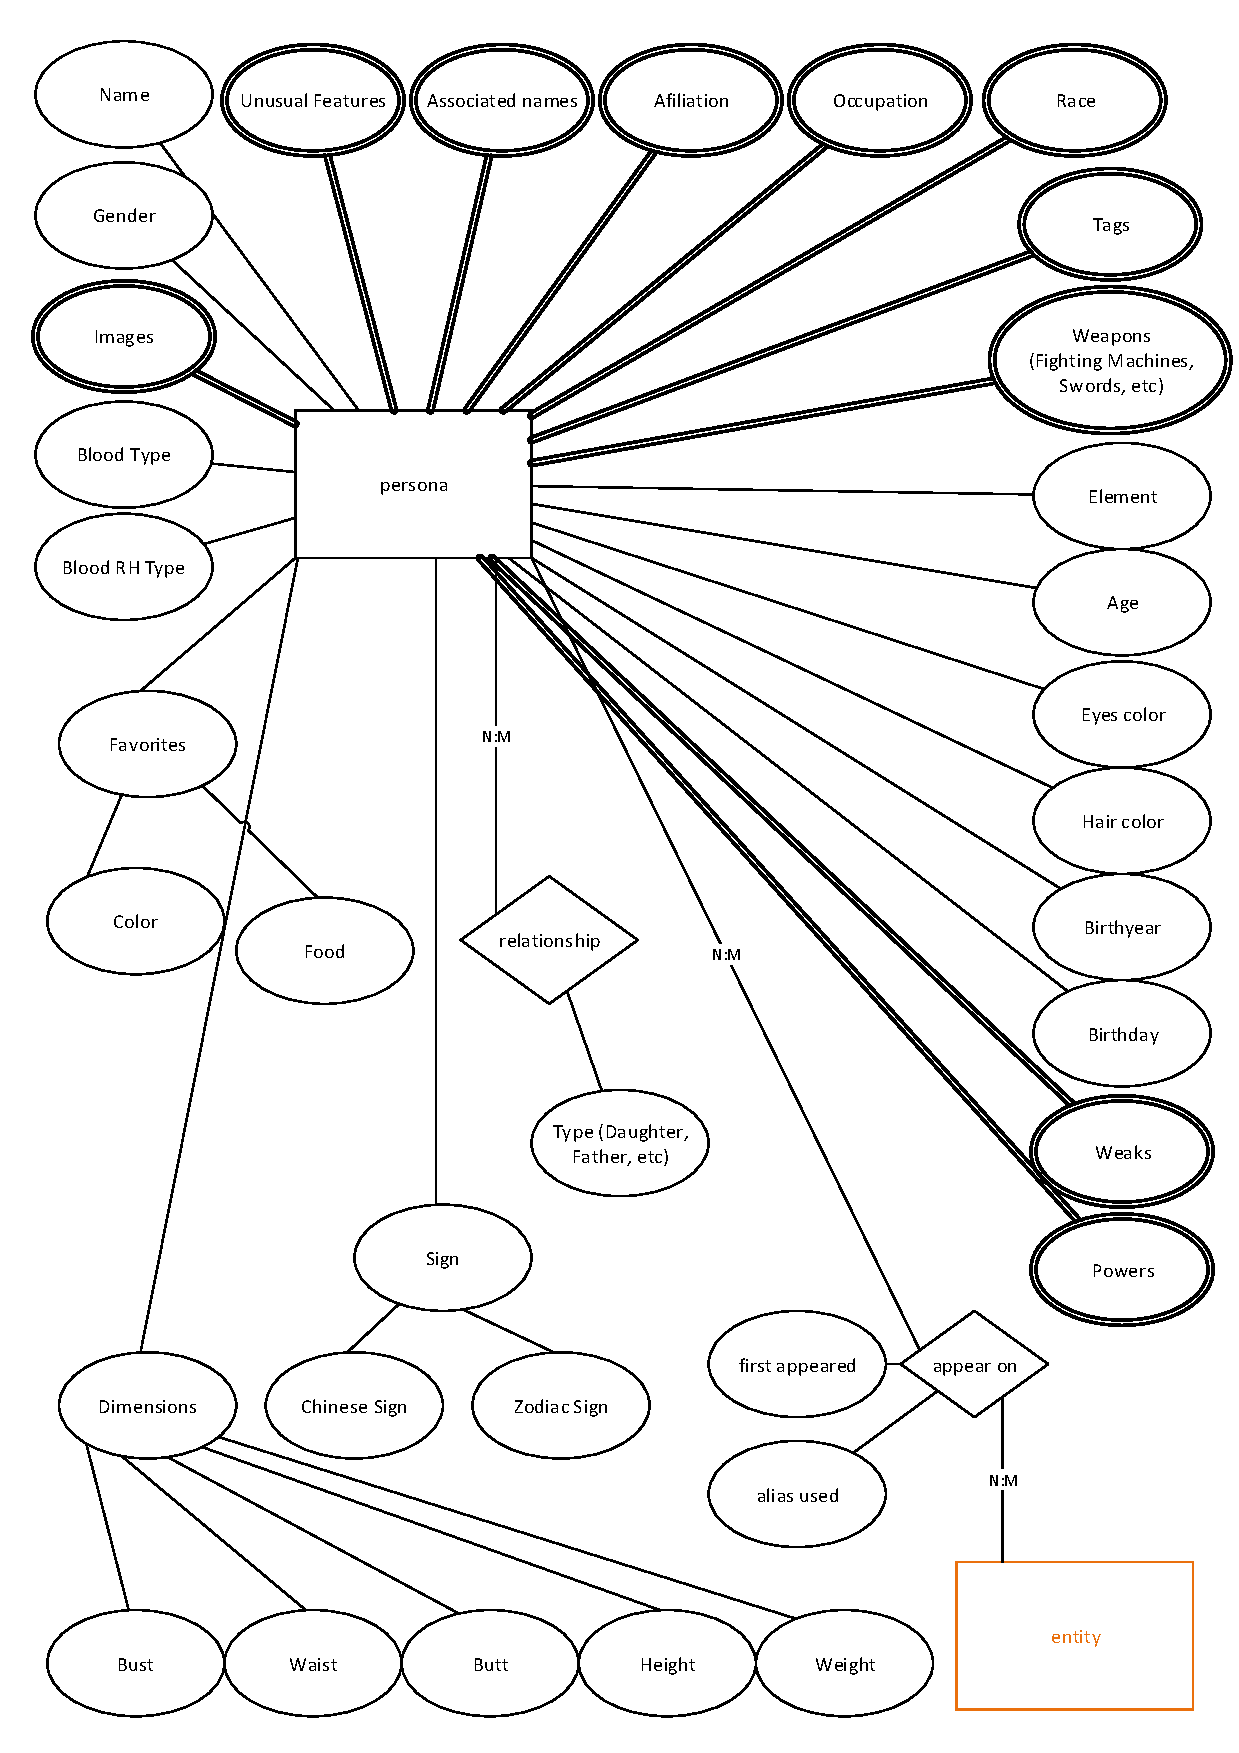
\includegraphics[width=.80\textwidth]{MER_-_Persona.pdf}
\caption{} \label{Persona}
\end{figure}


Como exemplo de Associação temos o relacionamento entre pessoas que dublam animações, animações dubladas e edições dubladas que são associadas ao número da edição, para situações onde o dublador oficial não pode dublar um episodio ou uma lista de episodios por motivos fora de seu controle. 

\begin{figure}[H]
\centering
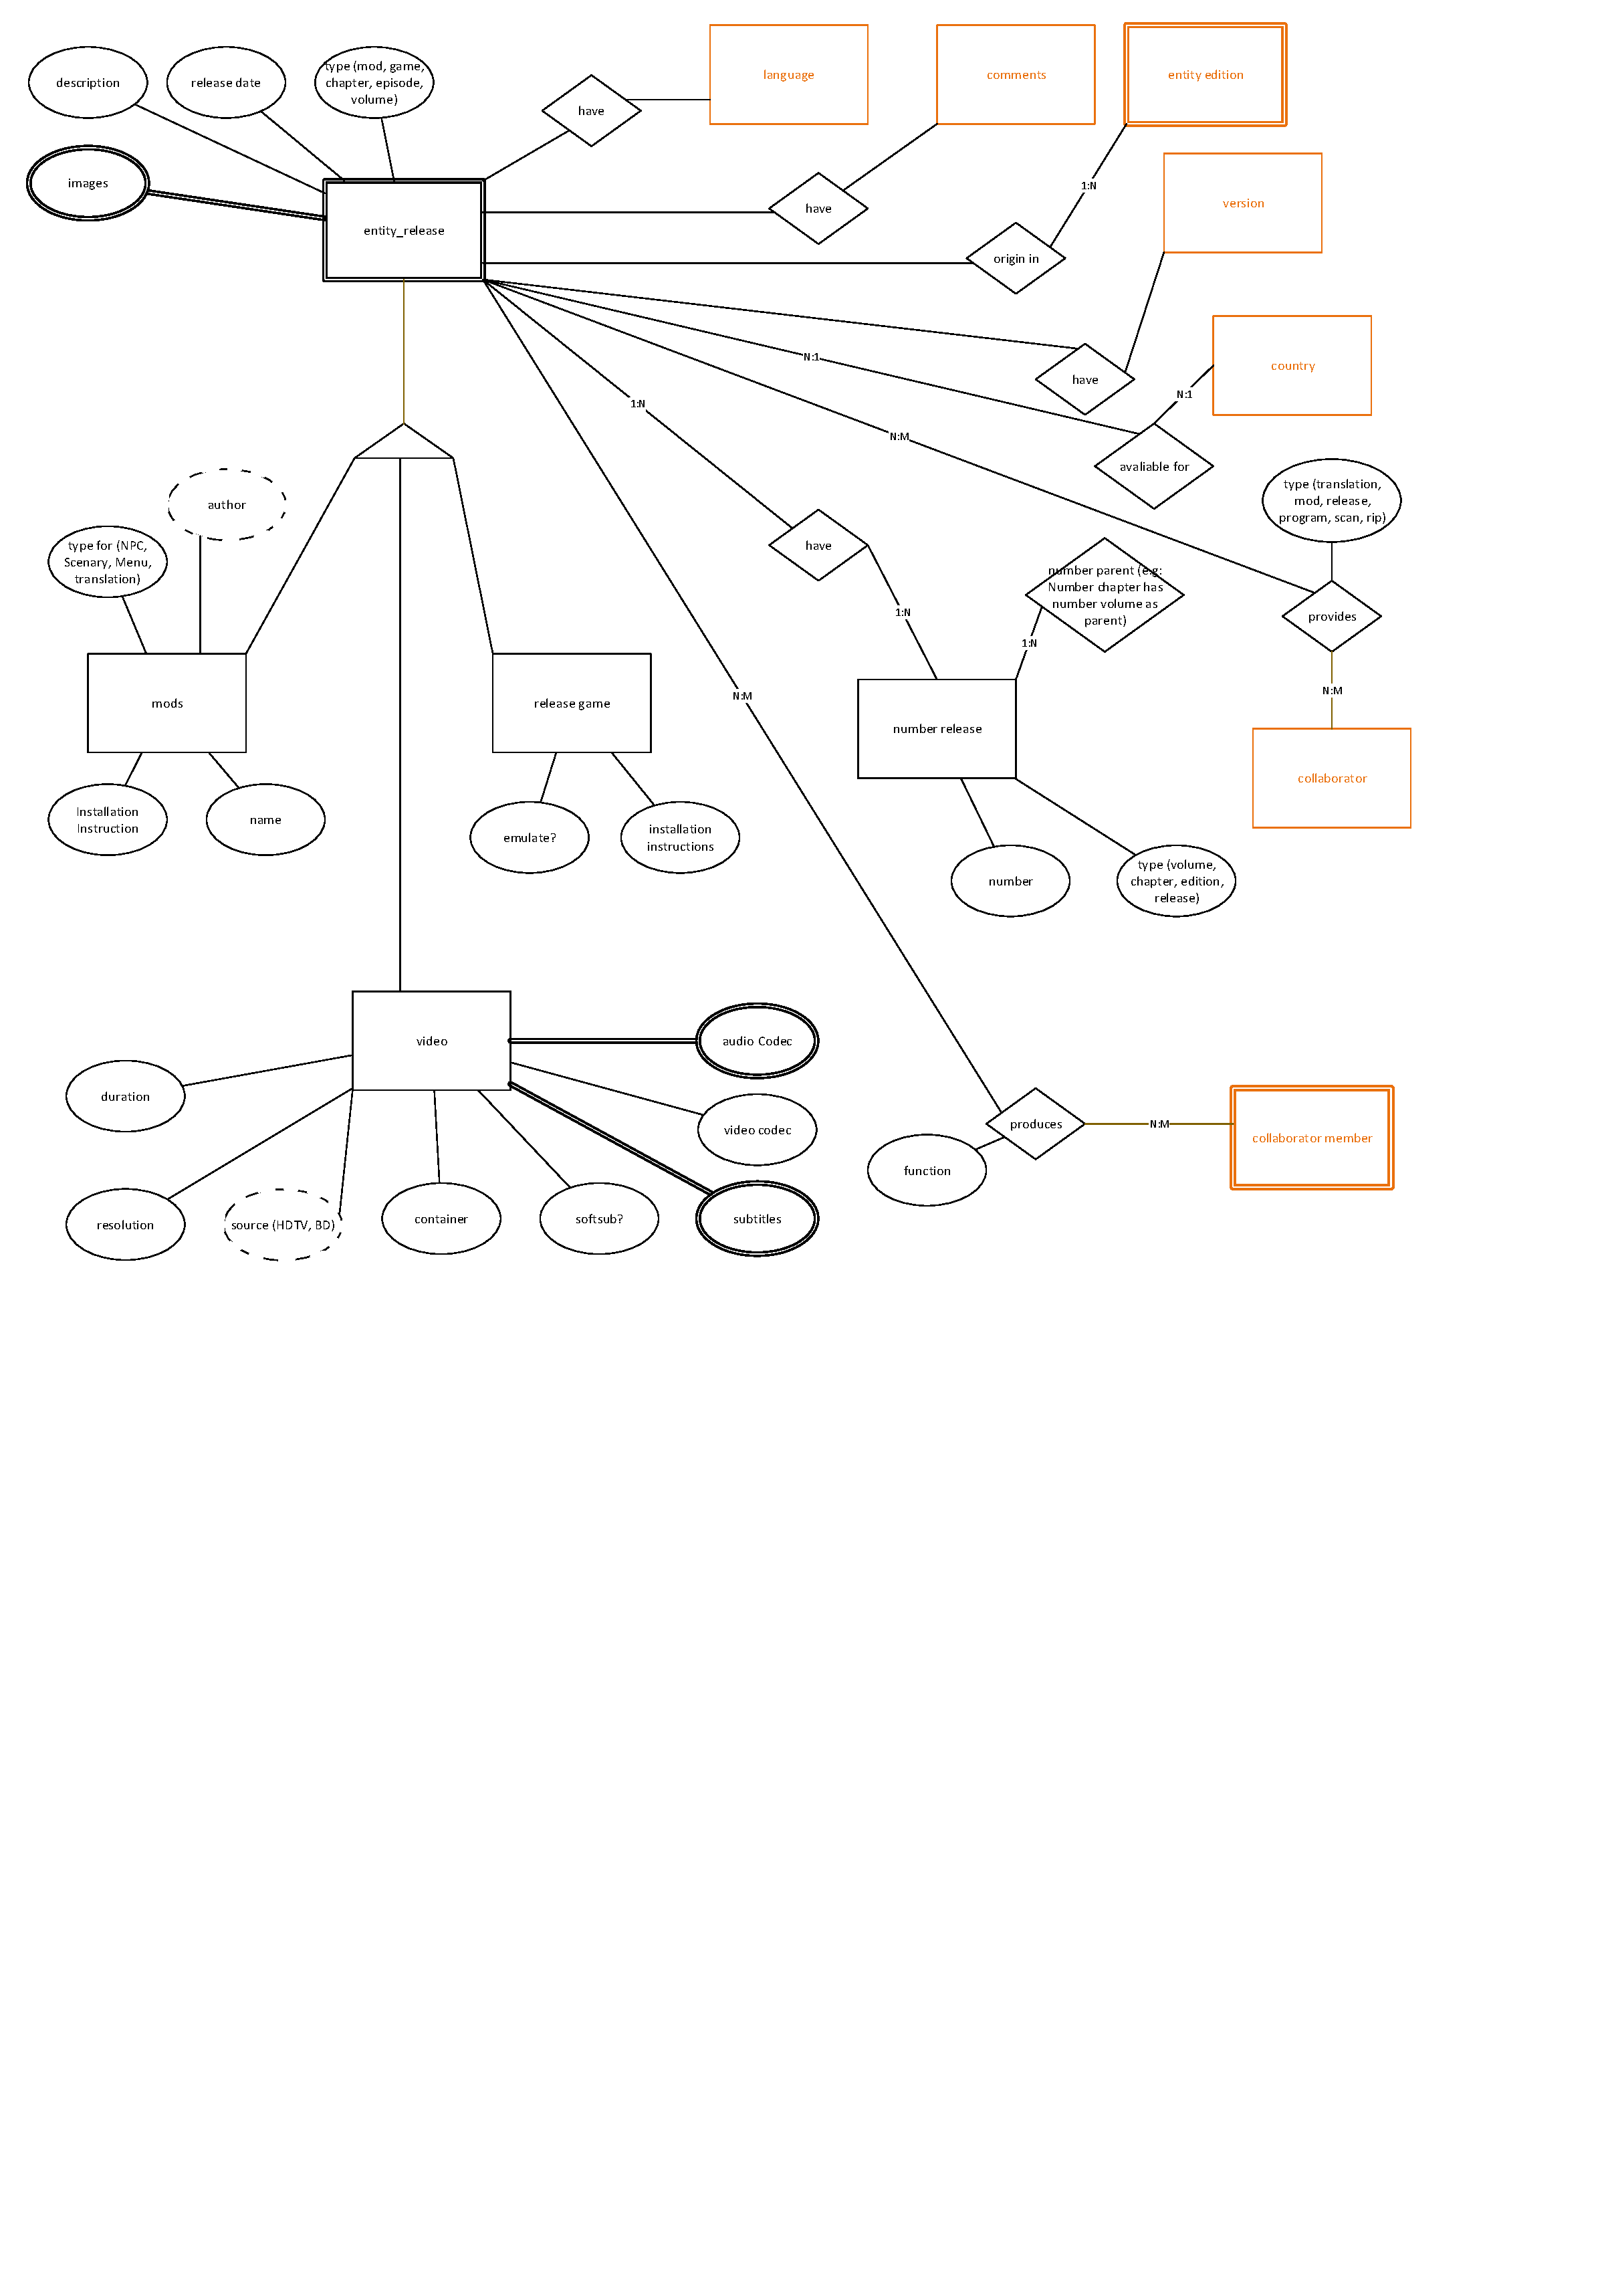
\includegraphics[width=.80\textwidth]{MER_-_Release.pdf}
\caption{Entidades responsáveis pelo armazenamento de conteúdo disponibilizado na web como modificações de jogos, conhecidos pela abreviação Mod, e traduções não oficiais de conteúdo ainda não licenciado fora do Japão.} \label{Release}
\end{figure}

\begin{figure}[H]
\centering
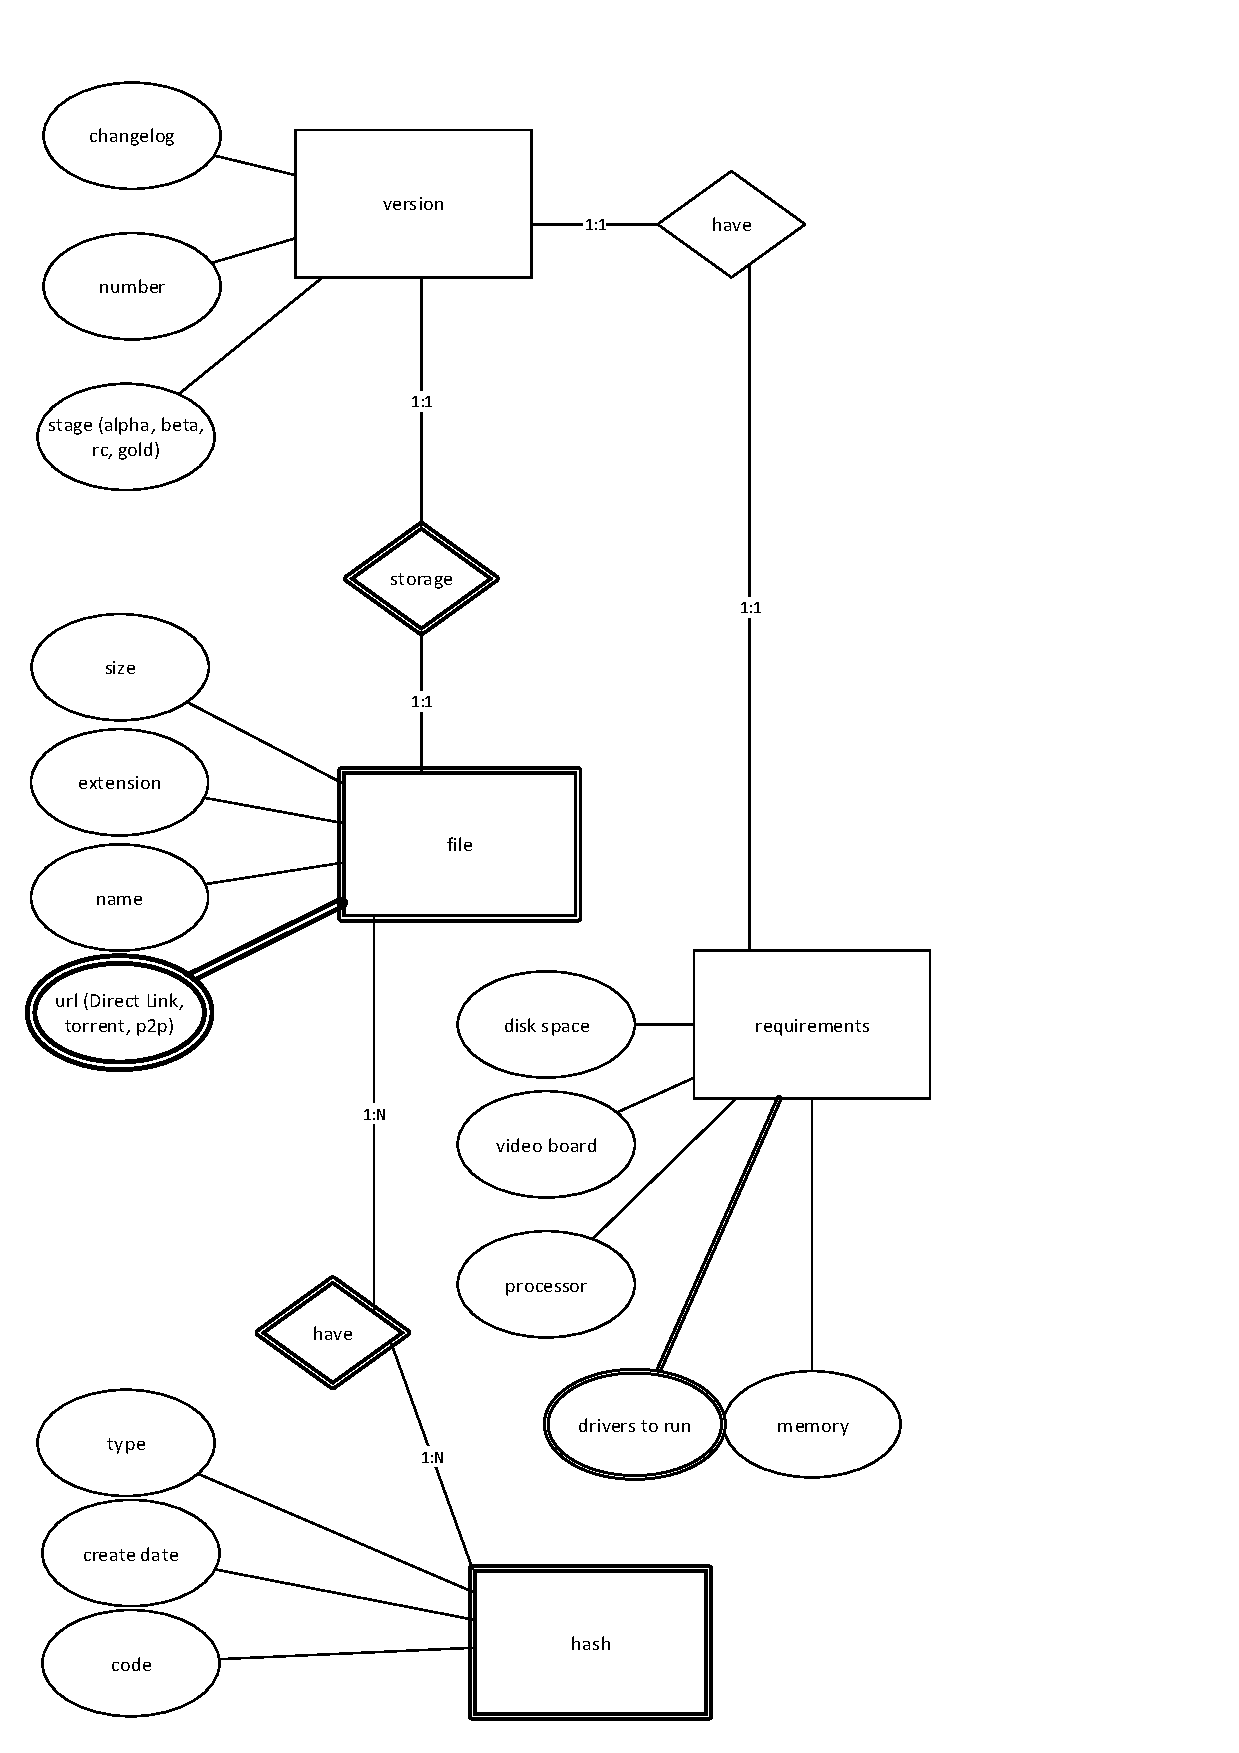
\includegraphics[width=.80\textwidth]{MER_-_Version.pdf}
\caption{Entidades responsáveis pelo armazenamento de informações de versões existentes de softwares, animações e livros e seus respectivos arquivos disponibilizados na web.} \label{hash}
\end{figure}


\begin{figure}[H]
\centering
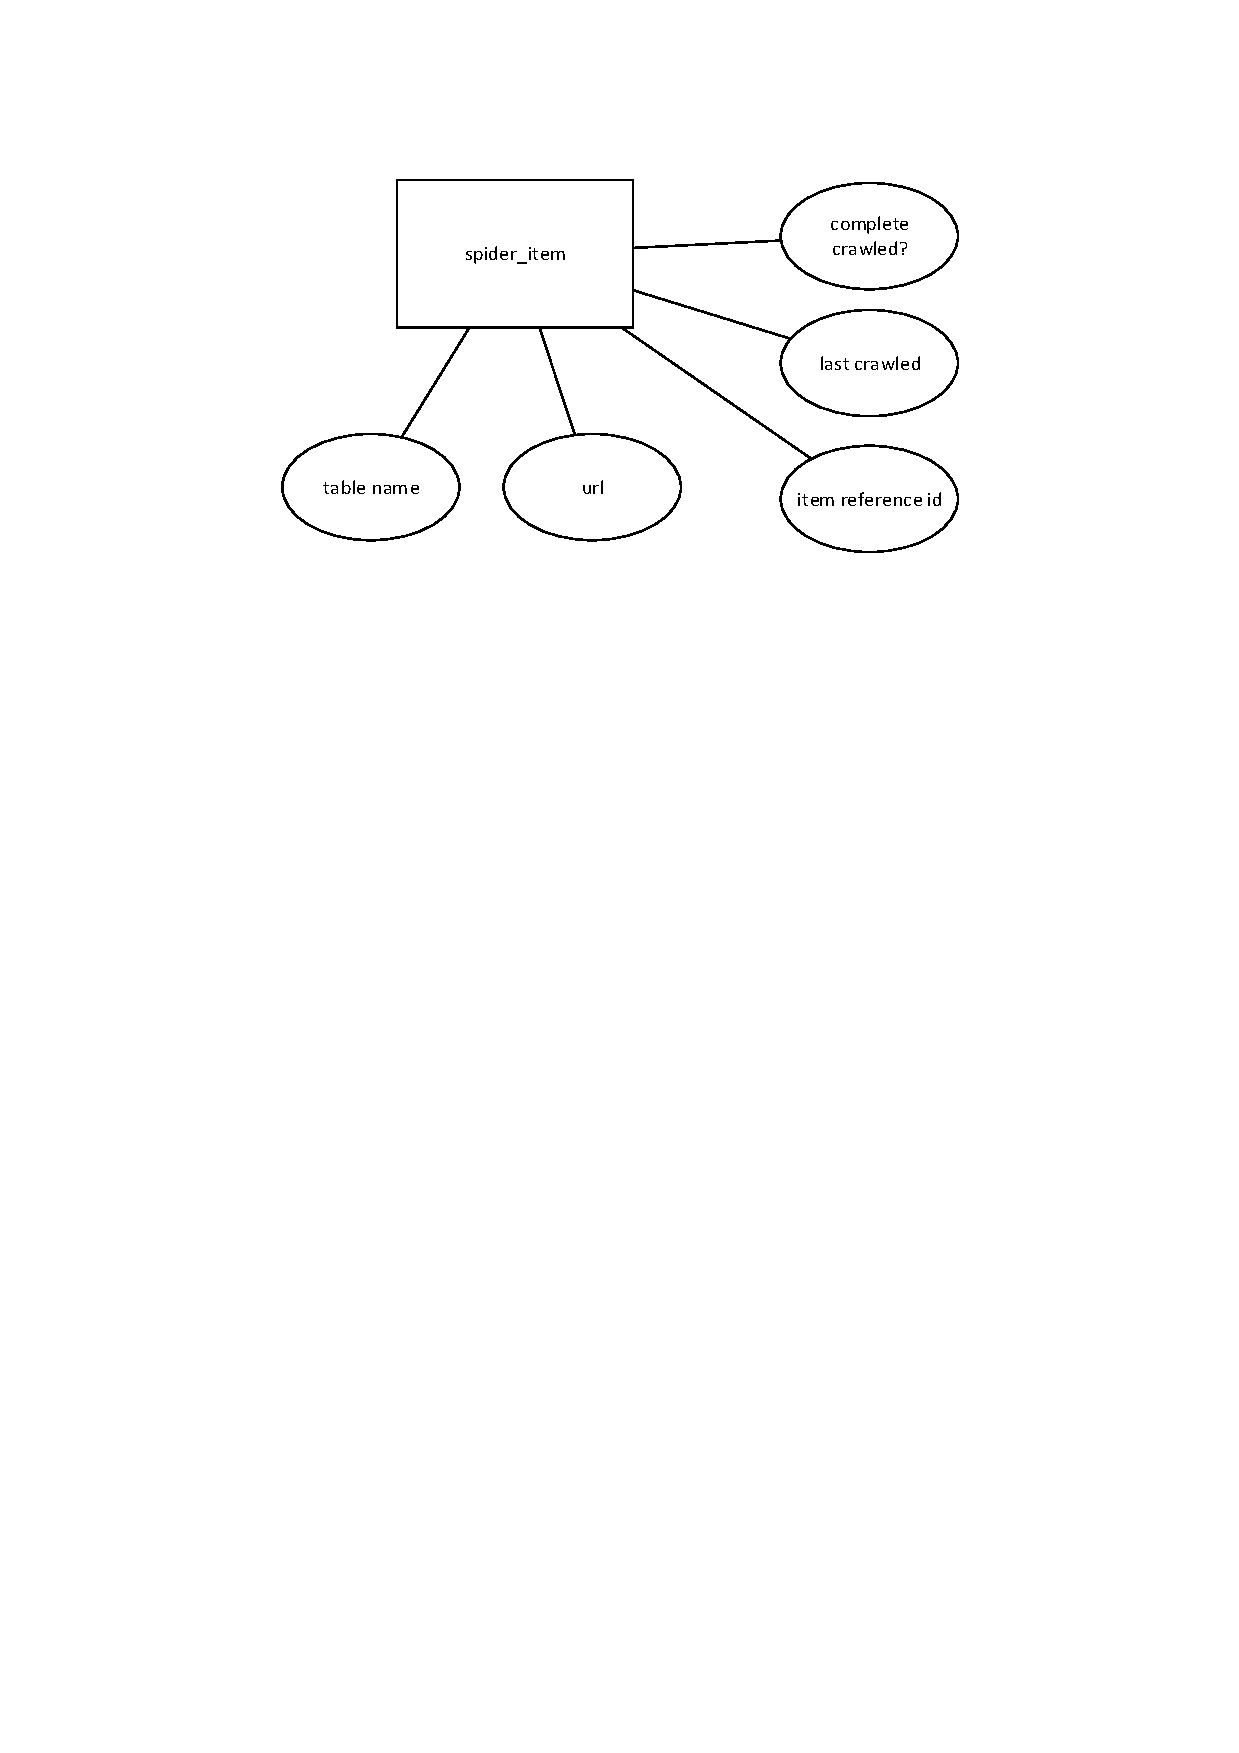
\includegraphics[width=.80\textwidth]{MER_-_Spider_item.pdf}
\caption{Entidade utilizada para se ter um controle das URL visitadas com as tabelas em que foram salvas as informações da URL e o ID correspondente nessas tabelas. Essa entidade não é utilizada para verificar se uma URL já foi visitada durante uma execução do Crawler e sim para verificar o ID relacionado e a última vez que as informações referentes ao ID foram atualizadas.} \label{hash}
\end{figure}

\subsubsection{Modelo Relacional}

Após a criação do Modelo Conceitual foram criadas as tabelas e relacionamentos do Modelo Relacional seguindo as três Formas Normais, separando portando atributos multi-valorados, não relacionados a totalidade da chave primaria em tabelas próprias quando necessário.

Também foram criadas chave-primarias não naturais, como índice numérico que serão auto incrementados na inserção de conteúdo, e definido valores padrões para atributos que armazenam Data e Hora.

Para as entidades que possuem mais de um tipo de título ou descrição como "Entity", "Persona" e "People" que possuem o tipo de título principal e alias foram criadas entidades para armazenamento desses títulos ou descrições com atributos que definem também o idioma do título ou descrição.


\subsubsection{Ferramentas Utilizadas para Modelagem}

Modelagem Conceitual

Para a modelagem do Banco de Dados e criação do Modelo Conceitual foi escolhido o Microsoft Visio que permite a geração de diversos tipos de diagramas, possibilitando a criação de novos itens se necessários para uso nos diagramas. Alguns dos itens como Associação, Atributos Compostos não estão presentes por padrão na modelagem de dados que vem com o Microsoft Visio e tiveram que serem criadas.

Modelo Relacional

Para o Modelo Relacional foi utilizado o DBDesign na sua 4ª versão, que permite a migração do Modelo Relacional para código SQL do MySQL, porém o DBDesign se mostrou limitado ao não permitir o aumento na área útil em que as entidades poderiam ser adicionadas, para uma modelagem extensa como a do Banco de Dados desse projeto essa limitação dificultou a organização pela falta de espaço fazendo com que as entidades ficassem muito próximas umas das outras. Além dessa limitação a própria implementação em JAVA do DB Design apresenta problemas com a hibernação no Sistema Operacional Windows, ao se hibernar e retornar quando se tenta salvar ou exportar um arquivo no DBDesign o programa trava sendo necessário reniciar o computador para voltar a utilizar essas opções. Portanto não é recomendo o uso do DB Design para um modelo relacional extenso. 

Modelo Lógico

Para criação do Modelo Lógico foi exportado do DB Design as queries SQL de criação de tabelas e índices, além da associação de chaves-estrangeiras. 

Para execução do Modelo Lógico para o PostgreSQL foi utilizado o Pg Admin III, sendo necessário converter alguns atributos gerados pelo DB Design que são específicos para MySQL como "auto increment" e "DATETIME" que foram convertidos para "SERIAL" e "timestamp" respectivamente.


\subsubsection{Detalhes da Implementação do Modelo Lógico}

Ao exportar o código SQL e alterá-lo para os detalhes de implementação próprios do PostgreSQL, além da conversão de tipos de dados para os tipos utilizados pelo PostgreSQL também é possível criar novos tipos. Para armazenar as informações de gênero de pessoas criamos um tipo de atributo gender que recebe os valores "Feminino", "Masculino" ou "Indefinido".


Os índices foram separados para serem executados apenas após a criação das tabelas e seus relacionamentos.

Como nossa implementação utiliza muito a consulta aos campos do banco de dados além de criarmos índices para chaves estrangeiras também criamos índices para todos os campos em que poderíamos executar uma consulta, uma vez que espaço de armazenamento não possui uma limitação atualmente como possuia quando as formas Normais foram desenvolvidas.

Nas tabelas que armazenam informações de tipos, como "entity\_type" que armazena os tipos de entidades (Mangá, Light Novel, Animação, etc) ou "blood\_type" que armazena o tipo sanguíneo após inserção de alguns tipos, antes da execução do crawler, com uma chave-primaria númerica prédeterminada foi necessário alterar o próximo valor da sequência para que não ocorresse erros de restrição de chave-primária.  


\subsection{Crawler}

Um crawler é um programa que visita websites, segue seus links e extrai informações das páginas. Um crawler deve a partir de uma URL inicial seguir todas as URL presentes na página a fim de vasculhar o website, 
pode ser utilizados critérios para seguir essas URL, como por exemplo seguir URL apenas do domínio atual do site, excluindo websites externos de publicidade e redes sociais.

O Crawler na URL inicial faz o download do código HTML da página e extrai a informação "href" do atributo <a> e os coloca numa lista de processamento que será utilizada para analisar se o link deve ser seguido ou removido da lista. 
Para evitar o problema de loops infinitos quando uma página A possui um link para uma página B e a página B possui link para a página A, deve-se criar uma pilha de links já visitados para verificação.   
 
Neste projeto foi optado pelo uso de uma biblioteca de Crawler que permite o seguimento de URL de páginas e extração de informações sem ter que se preocupar em programar Request e Download de páginas da Web.

O Biblioteca escolhida foi o Scrapy, na versão 0.24.4, desenvolvida em Python, possibilitando a criação da lógica de links a serem seguidos usando regras conhecidas como Rules que salvam informações em expressão regular das características dos links a serem visitados ou a serem removidos da pilha de processamento.
 
Como os websites a serem utilizados possuem conteúdo estático sem uso de Ajax o Scrapy atende as necessidades básicas de download e parseamento de websites. Se for necessário extrair informações dinamicamente geradas por AJAX pode ser utilizado o Scrapy com extensão para Firefox ou outra biblioteca de Crawler que permite o download do código-fonte da página como visualizado pelos browser, como a biblioteca Selenium.

Scrapy assim como Python está disponível para Windows e Linux.

\subsubsection{Links Duplicados}

Ao se desenvolver um crawler um dos problemas encontrados que deve ser evitado é o loop inesperado que ocorre quando uma página visitada possui uma URL para uma página anteriormente visitada. Para evitar situações como essa os links visitados devem ser armazenados, a cada link extraído pelo Crawler da página deve ser verificado se já não foi visitado antes de seguir ou não o link fazendo download da nova página. 
A biblioteca Scrapy já lida com links duplicados, ela o faz criando uma "impressão digital" da URL visitada, ou seja, uma representação da URL e seus parâmetros, assim quando duas ou mais URLs com parâmetros com ordens diferentes levam a um mesmo local um deles será considerado como visitado pois a "impressão digital" já foi visitada. A "impressão digital" de uma URL é criada extraindo a informação dos parâmetros e reordenando a URL, assim mesmo que URL possuem ordens diferentes a impressão digital possuirá uma única ordem. 

\subsubsection{Projeto Scrapy}

Scrapy é uma biblioteca com todos os recursos disponíveis para extrair informações de um website, utilizando Requests e Parse para download de websites e parseamento das informações. Os Requests e Parses são realizados por meio de classes conhecidas como Spider.

Um novo projeto Scrapy pode ser iniciado pela linha de comando e ao ser iniciado será criado uma estrutura pronta de pastas e arquivos padrões com algumas configurações pré-determinadas.
 
"Estrutura de Pastas aqui"

Para a visitação de URLs e extração de dados dos websites Scrapy utiliza as classes spiders armazenadas na pasta "spiders", essas classes devem ser herdar de pelo menos um tipo de spider disponível no Scrapy, cada um com sua implementação única.

A classe que escolhemos herdar para criar nossos spiders é a CrawlSpider que implementa o método parse, método esse que utiliza as regras definidas para ou seguir uma URL ou efetuar parse da URL. Quando definimos as regras, em um objeto iterável com nome "rules" na classe, indicamos por meio de expressão regular as páginas que podem ser seguidas e as páginas que devem ter seu conteúdo extraído, parseado e enviado para um método callback. Pode apenas haver um método callback para extração de dados.

Nossa classe spider para ser corretamente executada pela biblioteca Scrapy deve informar a propriedade nome do "spider", dominios permitidos para extração de informação sem o schema "http", as URLs iniciais e as regras de visitação e extração de URL.

Ao criarmos o método callback podemos usá-lo de pelo menos dois modos: Usá-lo para armazenar as informações extraídas em objetos conhecidos como "items" para serem depois interpretados por diversos métodos "Pipeline" que verificarão se os "items" estão dentro de uma qualificação lógica adequada para serem salvos em Banco de Dados ou arquivos Json (Esse é o método recomendado pelo Scrapy). Ou usá-lo diretamente para salvar as informações sem a necessidade de criação de objetos items.

Adotamos esse último método na qual as URLs extraídas e parseadas possuem seus dados normalizados para serem salvos no Banco de Dados no próprio método callback.
 
 
 
 

\subsubsection{Implementando acesso ao Banco de Dados}

Para acesso ao Banco de Dados PostgreSQL foi utilizado a biblioteca Psycopg2 e criado 


\subsubsection{Efetuando Login antes de Crawlear}


\subsubsection{Tratamento de Erros e Transactions}






\subsection{Normalização dos Dados Salvos}

Após extrair os dados, esses foram analisados e salvos normalizados. Porém algumas informações só podem ser estipuladas após a obtenção de todos os dados.

Como exemplo temos o item que iniciou uma coleção, só pode ser estipulado a partir da data de lançamento dos itens integrantes da coleçao e só após todos os dados serem salvos podemos descobrir qual item é o mais antigo da coleção.




\subsubsection{1º Passo no Desenvolvimento}

Com a escolha da biblioteca para o crawler foram analisados os links das páginas escolhidas e definidos quais links seriam seguidos em busca de outros links para conteúdo assim como quais links seriam de conteúdo para parseamento. 



\subsubsection {Abordagens de Spiders}

Abordagem assincrona.

Sobreescrita de métodos para efetuar login, de métodos
Implementação de Requests na própria classe requer um tratamento diferenciado ao código, só pode existir uma chamada a Request no CrawlSpider, mais que isso e o CrawlSpider não consegue lidar com request e interrompe a busca =.



\subsection{Processamento e relacionamento de Dados}

Após a extração dos dados e inserção no Banco de dados, os dados precisariam ser ....


\subsection{Visualização de Dados}

\section{Resultados}

Resultados.
Quais foram os dados considerados? Qual é o volume desses dados? Quanto tempo foi
necessário para obtê-los e armazená-los? Quais visualizações foram consideradas interessantes e quais não
foram? Quanto tempo foi necessário para gerar essas visualizações? Alguma delas foi surpreendente?


\section{Conclusão}


\bibliographystyle{plain}
\begin{thebibliography}{2}

\end{thebibliography}
\end{document}